% This file was converted to LaTeX by Writer2LaTeX ver. 1.6.1
% see http://writer2latex.sourceforge.net for more info
\documentclass[a4paper,12pt]{jarticle}
\usepackage[utf8]{inputenc}
\usepackage{amsmath}
\usepackage{amssymb,amsfonts,textcomp}
\usepackage[T1]{fontenc}
\usepackage[english]{babel}
\usepackage{color}
\usepackage{array}
\usepackage{supertabular}
\usepackage{hhline}
\usepackage[dvipdfmx]{hyperref}
\usepackage{pxjahyper}
\usepackage{lastpage}
\hypersetup{colorlinks=true, linkcolor=blue, citecolor=blue, filecolor=blue, urlcolor=blue}
\usepackage[dvipdfmx]{graphicx}
\graphicspath{%
{./text04-img/}%
}
%\usepackage{svg}
\usepackage{bbding,pifont,wasysym,amssymb}
% Outline numbering
\setcounter{secnumdepth}{2}
\renewcommand\thesection{\arabic{section}}
\renewcommand\thesubsection{\arabic{section}.\arabic{subsection}}
\makeatletter
\newcommand\arraybslash{\let\\\@arraycr}
\makeatother
% Page layout (geometry)
\setlength\voffset{-1in}
\setlength\hoffset{-1in}
\setlength\topmargin{2cm}
\setlength\oddsidemargin{2cm}
\setlength\textheight{24.770668cm}
\setlength\textwidth{17.006cm}
\setlength\footskip{26.144882pt}
\setlength\headheight{0cm}
\setlength\headsep{0cm}
% Footnote rule
\setlength{\skip\footins}{0.12cm}
\renewcommand\footnoterule{\vspace*{-0.018cm}\setlength\leftskip{0pt}\setlength\rightskip{0pt plus 1fil}\noindent\textcolor{black}{\rule{0.25\columnwidth}{0.018cm}}\vspace*{0.102cm}}
% Pages styles
\makeatletter
\newcommand\ps@Standard{
  \renewcommand\@oddhead{}
  \renewcommand\@evenhead{}
  \renewcommand\@oddfoot{ \hspace{80mm} 子どもIT未来塾~~第4回 \hfill \thepage\ / \pageref{LastPage}}
  \renewcommand\@evenfoot{\@oddfoot}
  \renewcommand\thepage{\arabic{page}}
}
\newcommand\ps@FirstPage{
  \renewcommand\@oddhead{}
  \renewcommand\@evenhead{}
  \renewcommand\@oddfoot{}
  \renewcommand\@evenfoot{\@oddfoot}
  \renewcommand\thepage{\arabic{page}}
}
\makeatother
\pagestyle{Standard}
\setlength\tabcolsep{1mm}
\renewcommand\arraystretch{1.3}

% List styles
\newcounter{saveenum}
\newcounter{Figure}
\renewcommand\theFigure{\arabic{Figure}}

\title{\Huge\bf 子どもIT未来塾 第4回}
\author{
\huge\bf プログラムで、いろいろ自動化してみよう
\vspace{15mm}
}
\date{ \Huge おにたま(武田 寧) 先生 }
\begin{document}
\clearpage\setcounter{page}{1}\pagestyle{Standard}
\thispagestyle{FirstPage}

\maketitle

\setcounter{page}{1}\pagestyle{Standard}

  % First Part:

\clearpage

\section{今回の授業}
\subsection{目標}
\ \ \ \ 対戦できるゲームで遊んでみよう

\ \ \ \ センサーのプログラムを作ろう

\subsection{授業内容}
%\liststyleLii
\begin{enumerate}
\item プログラミングの復習をしよう
\item 対戦ゲームで遊んでみよう
\item センサーボードをプログラムで使おう
\item ゲームの動きを改造してみよう
\end{enumerate}
\subsection{注意点}
%\liststyleLiii
\begin{itemize}
\item
授業の合間のきゅうけいでは、遠くのものをながめたりして目を休めましょう
\item 水分ほきゅうはこまめにしましょう
\item
先生が説明中は先生の話を聞きましょう
\item
わからないことがあったらTAの先生方にすぐ聞きましょう
\end{itemize}

\subsection{ラズベリーパイを使うときの注意}
%\liststyleLvii
\begin{itemize}
\item
水などぬれているものをラズベリーパイ本体につけないようにしましょう
\end{itemize}
%\liststyleLviii
\begin{itemize}
\item
ラズベリーパイをはじめコンピュータなどは熱に弱いのですごく暑い部屋では使わないようにしましょう
\end{itemize}
%\liststyleLix
\begin{itemize}
\item
ラズベリーパイなどは静電気によわいので注意しましょう
\end{itemize}
%\liststyleLx
\begin{itemize}
\item
ラズベリーパイをらんぼうに扱うのはやめましょう
\end{itemize}
%\liststyleLxi


  % Main Part:

\clearpage
\section{プログラミングの復習をしよう}


\subsection{作業フォルダの準備}
\bigskip
\bigskip

上にあるバーのアイコンからファイルマネージャーを開いてみましょう。

\bigskip
\bigskip

\begin{minipage}{9.781cm}
\centering
{\upshape
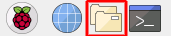
\includegraphics[keepaspectratio,width=5.898cm,height=1.242cm]{text04-img/text02-img001.png}
\flushleft

Figure \stepcounter{Figure}{\theFigure}: ファイルマネージャーを開くアイコン}
\end{minipage}

\bigskip
\bigskip
\bigskip

これから作業で使うファイルをコピーしてもらいます。「/home/ユーザー名」のフォルダに、第4回で使うフォルダ「04」をコピーすることから始めます。

まず、「/usr/local/share/ome」という場所を開いてみましょう。

どこにあるか探すことができますか?

わからない時は、TAや先生に聞いてみましょう。

\bigskip
\bigskip

\begin{minipage}{9.781cm}
\centering
{\upshape
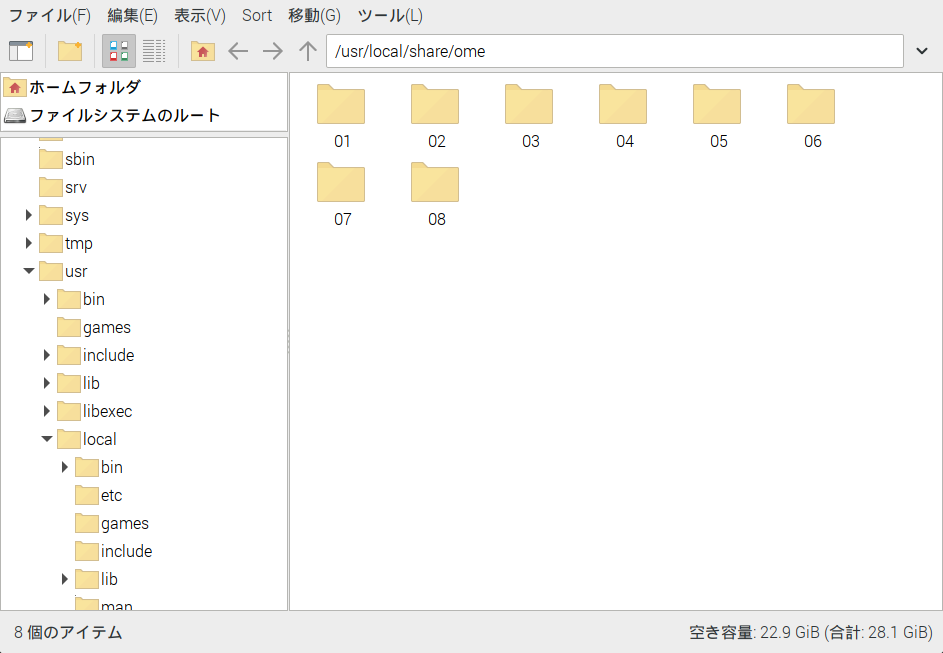
\includegraphics[keepaspectratio,width=11.232cm,height=8.424cm]{text04-img/s_ome04a.png}
\flushleft

Figure \stepcounter{Figure}{\theFigure}: /usr/local/share/ome フォルダ}
\end{minipage}

\bigskip
\bigskip
\bigskip

この中に、「04」という名前のフォルダがあります。これから、この「04」というフォルダを自分の作業フォルダにコピーします。

「04」という名前のフォルダ上でマウスの右クリックを押して「コピー」を選んでください。

\bigskip
\bigskip

\begin{minipage}{9.781cm}
\centering
{\upshape
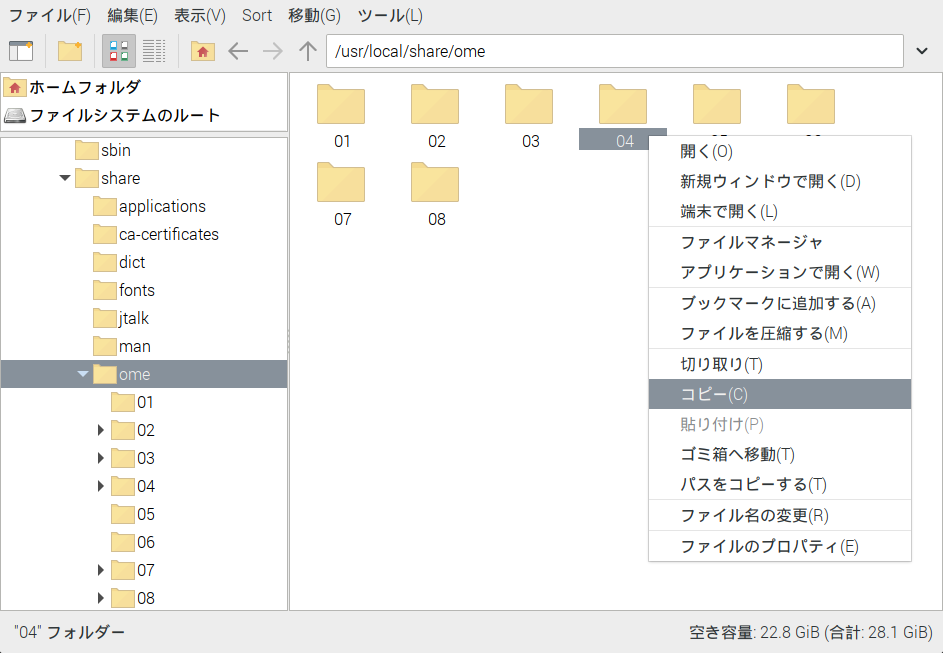
\includegraphics[keepaspectratio,width=11.232cm,height=8.424cm]{text04-img/s_ome04b.png}
\flushleft

Figure \stepcounter{Figure}{\theFigure}: 04フォルダでコピーを選ぶところ}
\end{minipage}

\bigskip
\bigskip
\bigskip

コピーを選ぶだけでは何も起こりません。この後、コピーしたい場所を選びます。

コピー先の場所は、「/home/ユーザー名」のフォルダになります。

たとえば、ユーザー名が「ome」だった場合は、「/home/ome」という場所にコピーします。

コピー先の場所を開いたら、何もない場所でマウスの右クリックを押して「貼り付け」を選んでください。

\bigskip
\bigskip

\begin{minipage}{9.781cm}
\centering
{\upshape
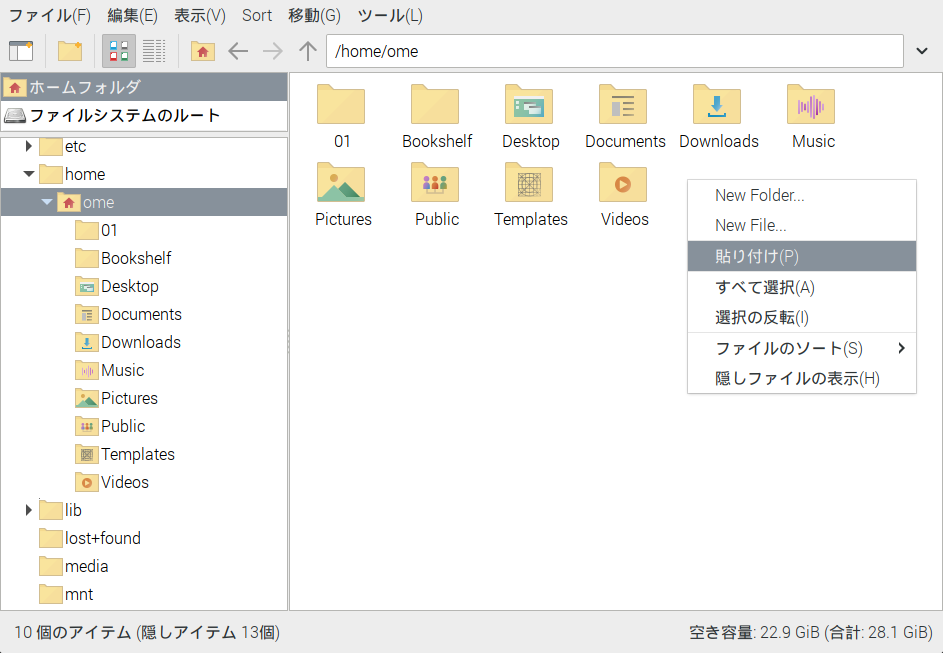
\includegraphics[keepaspectratio,width=11.232cm,height=8.424cm]{text04-img/s_ome04c.png}
\flushleft

Figure \stepcounter{Figure}{\theFigure}: 04フォルダでコピーを選ぶところ}
\end{minipage}

\bigskip
\bigskip
\bigskip

これで先ほどの「/usr/local/share/ome/04」フォルダが、「/home/ユーザー名/04」にコピーされます。

ファイルには、画像や文章、音声や動画など、さまざまなデータが入っています。

これから皆さんが作業で使うファイルは、「/home/ユーザー名/04」という場所に置かれています。

ファイルの中身が何なのか、自分が作ったファイルかどうかを知っておいてください。

\bigskip
\bigskip

\begin{minipage}{9.781cm}
\centering
{\upshape
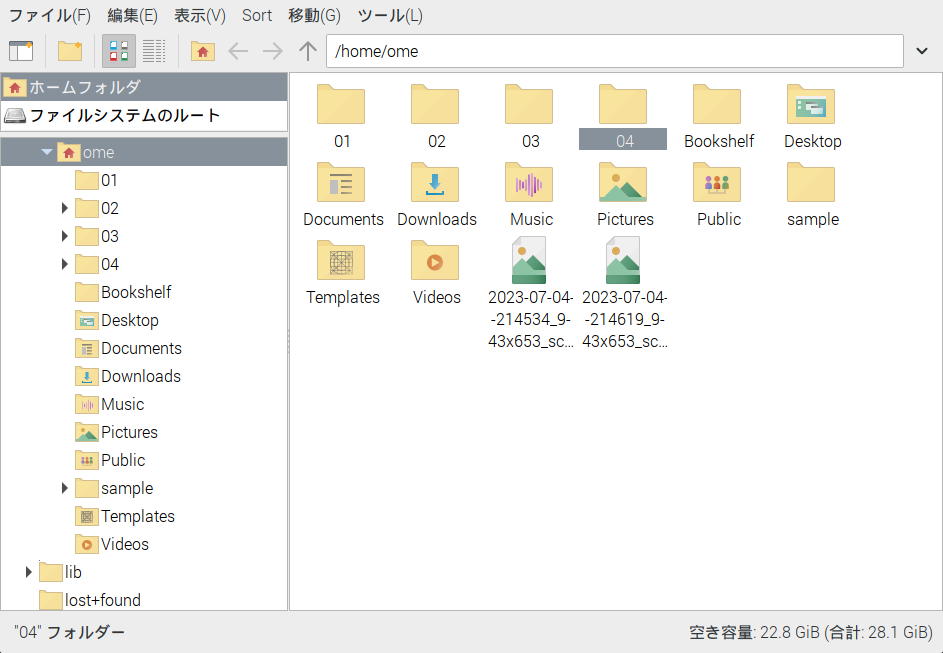
\includegraphics[keepaspectratio,width=11.232cm,height=8.424cm]{text04-img/s_ome04d.png}
\flushleft

Figure \stepcounter{Figure}{\theFigure}: 04フォルダがコピーされた画面}
\end{minipage}

\bigskip
\bigskip
\bigskip





\clearpage
\subsection{条件判断の使い方}
\bigskip
\bigskip

今回もまず、プログラミングのツールHSP(Hot Soup Processor)を起動して、プログラムを実行するための準備を始めましょう。左上のRaspberry Piメニューの「プログラミング」項目にある、「HSP Script Editor」(HSPスクリプトエディタ)からエディタを起動してください。

\bigskip
\bigskip

\begin{minipage}{9.781cm}
\centering
{\upshape
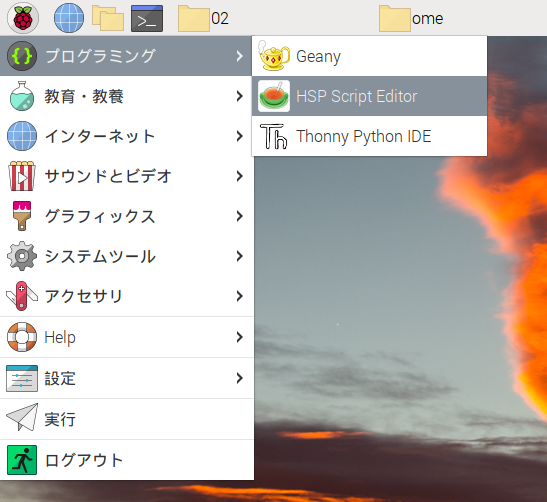
\includegraphics[keepaspectratio,width=7.31cm,height=6.562cm]{text04-img/s_hspmenu.png}
\flushleft

Figure \stepcounter{Figure}{\theFigure}: プログラミング項目のメニュー}
\end{minipage}

\bigskip
\bigskip
\bigskip

いつも通りに、HSPスクリプトエディタを起動して作業を始めていきましょう。


\bigskip
\bigskip

\begin{minipage}{9.781cm}
\centering
{\upshape
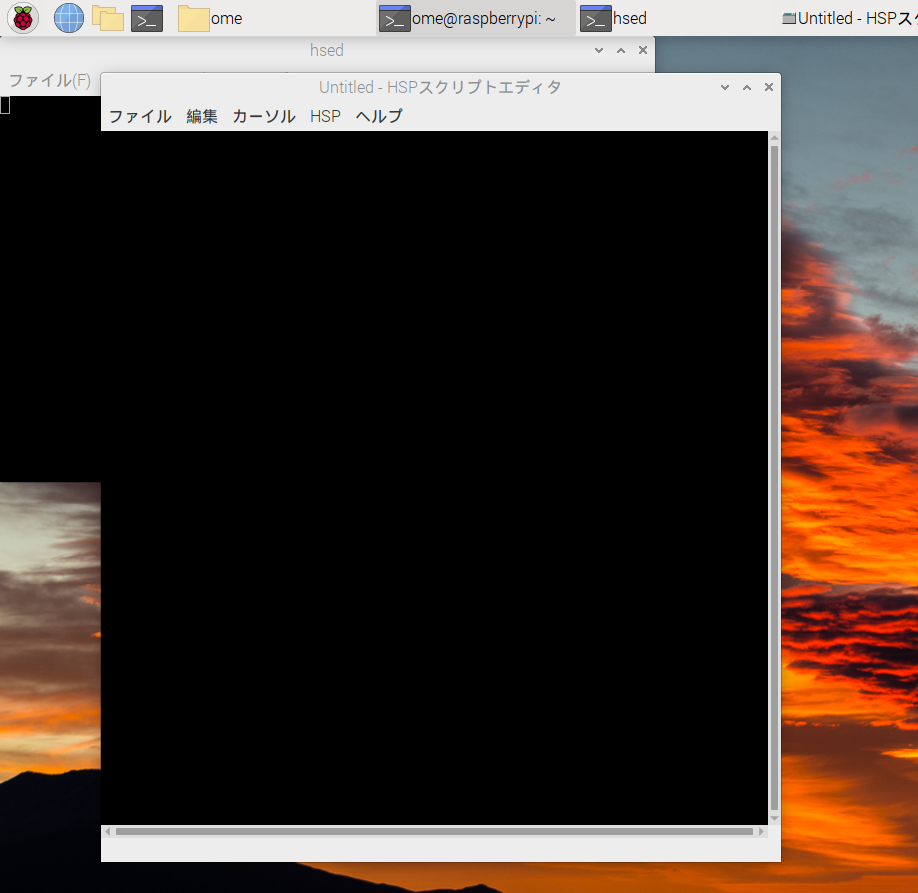
\includegraphics[keepaspectratio,width=7.31cm,height=6.562cm]{text04-img/s_hsed.png}
\flushleft

Figure \stepcounter{Figure}{\theFigure}: HSPスクリプトエディタを起動したところ}
\end{minipage}

\bigskip
\bigskip
\bigskip

まずは、教材のプログラムを動かして試してみましょう。

ファイル→「開く」メニューから /home/ユーザー名/04 フォルダの中にある「swhandan.hsp」を読み込んでください。
作業は、すべて「/home/ユーザー名/04」フォルダで行ないます。

見つからない場合は、まわりの友達か、近くの先生に聞いてみてください。


\bigskip
\bigskip

\begin{minipage}{9.781cm}
\centering
{\upshape
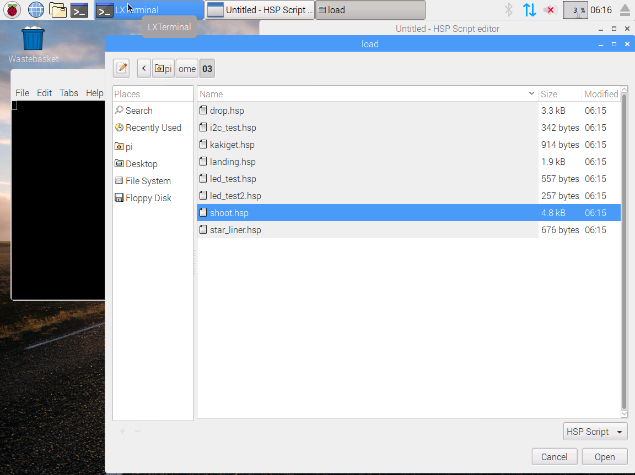
\includegraphics[keepaspectratio,width=7.338cm,height=5.493cm]{text04-img/text04-img002.png}
\flushleft

Figure \stepcounter{Figure}{\theFigure}: フォルダから読み込む画面}
\end{minipage}

\bigskip
\bigskip
\bigskip

「swhandan.hsp」は、センサーボード上のスイッチを押すとメッセージが変わるかんたんなプログラムです。早速、[F5]キーを押して実行してみましょう。

\bigskip
\bigskip

\begin{minipage}{9.781cm}
\centering
{\upshape
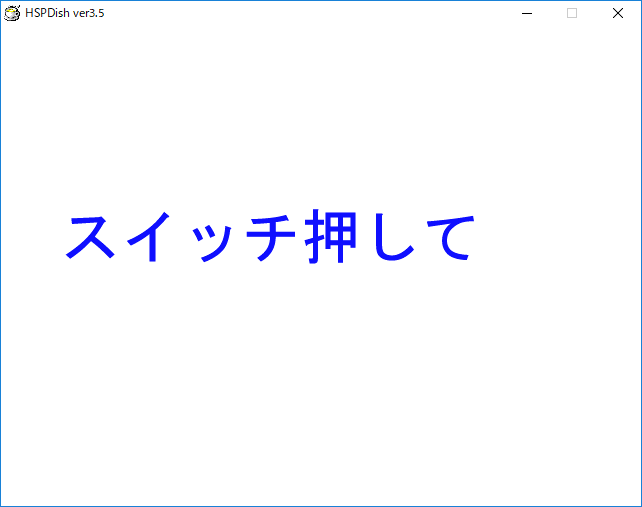
\includegraphics[keepaspectratio,width=7.673cm,height=6.05cm]{text04-img/text04-img003.png}
\flushleft

Figure \stepcounter{Figure}{\theFigure}: swhandan.hspの実行画面}
\end{minipage}

\bigskip
\bigskip
\bigskip

\clearpage
\bigskip
\bigskip
第2回で出てきた条件判断について思い出してみましょう。

プログラムは最初の行から、下に向かって順番に実行されます。実際には、一瞬で過ぎてしまうのでわかりにくいですが、どのような順番でコンピューターが動くのか、想像しながら見てみることが大切です。わからない命令は以前の講座を復習してみましょう。

「*hata」から「goto *hata」までの間が「スイッチ押して」という文字を表示する部分です。

\bigskip

{\bfseries
*hata}

{\bfseries
\ \ redraw 0}

{\bfseries
\ \ font {\textquotedbl}{\textquotedbl},60}

{\bfseries
\ \ pos 60,180}

{\bfseries
\ \ color 0,0,255}

{\bfseries
\ \ mes {\textquotedbl}スイッチ押して{\textquotedbl}}

{\bfseries
\ \ redraw 1}

{\bfseries
\ \ await 16}

{\bfseries
\ \ if gpioin(5)=0 : goto *hata2}

{\bfseries
\ \ goto *hata}


\bigskip

ここでセンサーボードのスイッチを押すと流れが変わります。


\bigskip

{\bfseries
*hata2}

{\bfseries
\ \ redraw 0}

{\bfseries
\ \ font {\textquotedbl}{\textquotedbl},60}

{\bfseries
\ \ pos 60,180}

{\bfseries
\ \ color 255,0,0}

{\bfseries
\ \ mes {\textquotedbl}押しましたね!{\textquotedbl}}

{\bfseries
\ \ redraw 1}

{\bfseries
\ \ await 16}

{\bfseries
\ \ if gpioin(6)=0 : goto *hata}

{\bfseries
\ \ goto *hata2}


\bigskip

「*hata2」から「goto *hata2」までの間で「押しましたね」という文字を表示しています。

それぞれの切り替えにスイッチを使っていますが、そのために条件判断を使っています。

スイッチの状態などを知る場合は、gpioinという関数を使います。


\bigskip

{\bfseries
\ \ 変数 = gpioin(GPIO番号)}

\bigskip

と書くことで、指定されたGPIO番号のスイッチがONかOFFかを調べることができます。


\bigskip
\bigskip

\begin{minipage}{9.781cm}
\centering
{\upshape
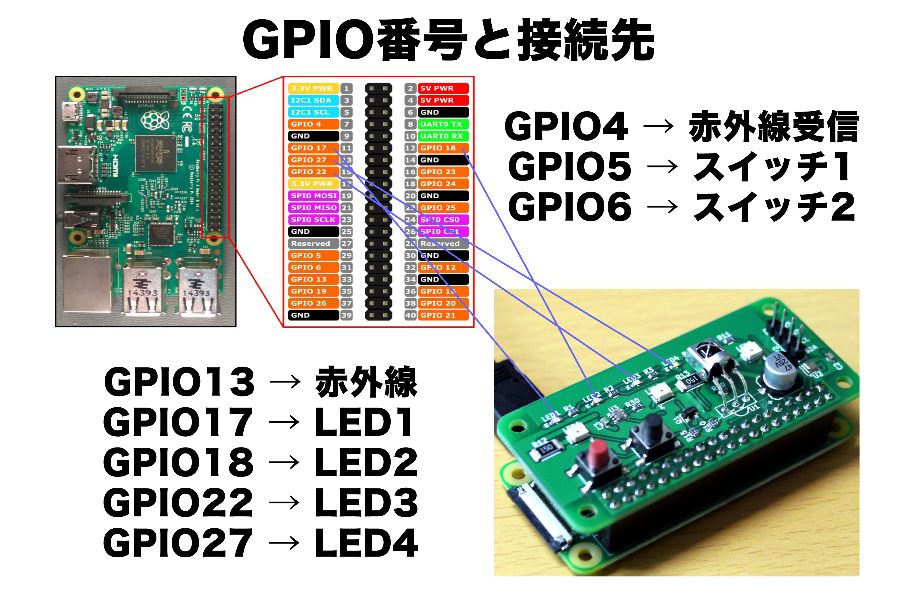
\includegraphics[keepaspectratio,width=12.409cm,height=7.62cm]{text04-img/text04-img004.png}}
\end{minipage}

\bigskip
\bigskip
\bigskip

スイッチが接続されているGPIOの番号を指定することで変数に値が入ります。

\bigskip

{\bfseries
\ \ a = gpioin(5)}

\bigskip

と書くことで、スイッチ1がONならば0、OFFならば1が変数に代入されます。

変数に記憶されている0か1の数字をもとに、条件判断で違う動作をさせることができます。

条件判断のための if命令 を思い出してみましょう。

\bigskip
\bigskip
\bigskip

{\bfseries
\ \ (HSPのルール)


\bigskip

\ \ if命令により条件を判断することができる

\ \ ifの後にスペースに続けて条件式を指定します

\ \ その後で「:」に続けて条件が正しい時に実行される命令を書きます}


\bigskip

\ \ (条件式はいくつか書き方があります)


\bigskip

\ \ \ \ 条件式 \ \ \ \ \ \ \ \ \ 意味

\ \ \ \ {}-{}-{}-{}-{}-{}-{}-{}-{}-{}-{}-{}-{}-{}-{}-{}-{}-{}-{}-{}-{}-{}-{}-{}-{}-{}-{}-{}-{}-{}-{}-{}-{}-{}-{}-{}-{}-{}-{}-{}-{}-{}-{}-{}-{}-{}-{}-{}-{}-{}-{}-{}-

\ \ \ \ 変数名 =
数値\ \ 変数の内容と数値が同じである

\ \ \ \ 変数名 !
数値\ \ 変数の内容と数値が同じではない

\ \ \ \ 変数名 {\textless}
数値\ \ 変数の内容より数値の方が数が大きい

\ \ \ \ 変数名 {\textgreater}
数値\ \ 変数の内容より数値の方が数が小さい

\bigskip
\bigskip

つまり、

\bigskip

{\bfseries
\ \ a = gpioin(5)

\ \ if a=0 : goto *hata}

\bigskip

のように書くことで、変数aが0の時だけ「*hata」の場所から実行させることができます。

(センサーボードのスイッチは押された時に0の値になります。1ではないので注意しましょう。)


\bigskip
\bigskip


\clearpage
\subsection{ミニサッカーゲームで遊んでみよう}
\bigskip
\bigskip

文字と簡単な図形を使うだけでもゲームを作ることができます。実際にできあがっているプログラムを動かして試してみましょう。

スクリプトエディタの、ファイル→「開く」メニューから「kick.hsp」を読み込みましょう。

作業は、すべて「/home/ユーザー名/04」フォルダで行ないます。

見つからない場合は、まわりの友達か、近くの先生に聞いてみてください。


\bigskip

[F5]キーで実行すると、ミニサッカーゲームが動きます。

\bigskip
\bigskip

\begin{minipage}{9.781cm}
\centering
{\upshape
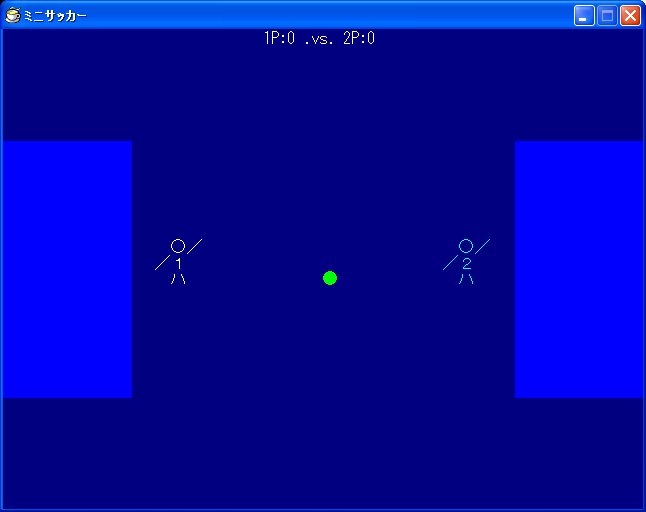
\includegraphics[keepaspectratio,width=9.075cm,height=7.197cm]{text04-img/text04-img005.png}
\flushleft

Figure \stepcounter{Figure}{\theFigure}: ミニサッカーゲームの画面}
\end{minipage}

\bigskip
\bigskip
\bigskip

このゲームは二人で対戦します。

隣の席にいる人と、2人1組になって一緒に遊んでみてください。

左側の「1」の人をキーボードの左側で操作します。


\bigskip

\ \ \ \ [W]

[A] \ \ \ \ [D] \ \ \ \ [S] = ゴール前にもどる

\ \ \ \ [X]


\bigskip


\bigskip


\bigskip

右側の「2」の人をキーボードの右側で操作します。


\bigskip

\ \ \ \ [↑]

[←] \ \ \ [→] \ \ \ \ [Enter] = ゴール前にもどる

\ \ \ \ [↓]


\bigskip

それぞれのプレイヤーは足でボールを蹴って遠くに飛ばすことができます。

\ \ \ \ 「1」の人は右のゴールへ、

\ \ \ \ 「2」の人は左のゴールへボールを入れたら点が入ります。

\bigskip

\ \ \ \ 3点先に取った人の勝ちです。

\ \ \ \ 同じグループの友達と対戦してみましょう。

\bigskip
\bigskip

\begin{minipage}{9.781cm}
\centering
{\upshape
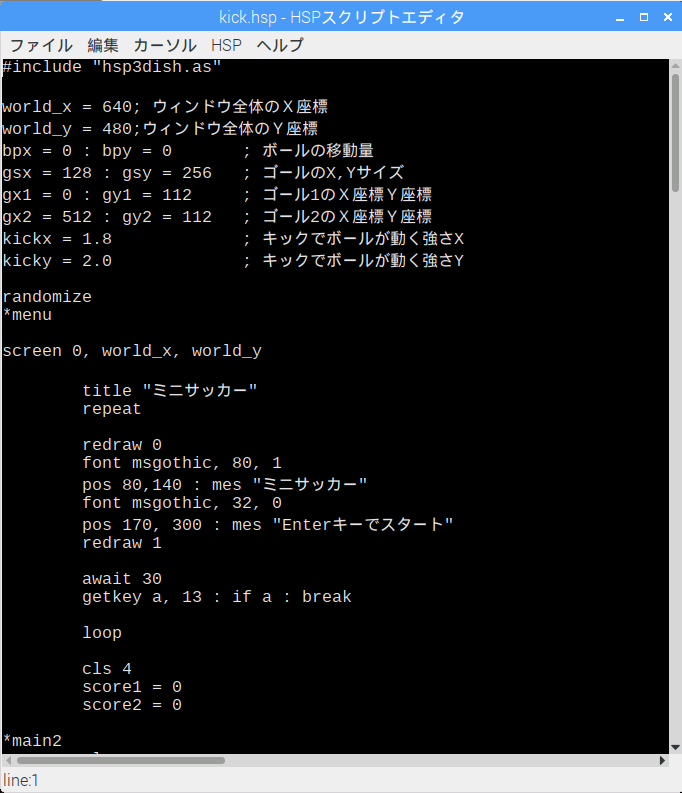
\includegraphics[keepaspectratio,width=9.657cm,height=11.229cm]{text04-img/text04-img006.png}
\flushleft

Figure \stepcounter{Figure}{\theFigure}: ミニサッカーゲームのプログラム}
\end{minipage}

\bigskip
\bigskip
\bigskip

\subsection{例題に挑戦しよう}

\bigskip
\bigskip

終わってしまった人は、以下の例題にも挑戦してみよう。

\bigskip

・ミニサッカーゲームの人を改造する

・ミニサッカーゲームのボールや色を変える

・ミニサッカーゲームの動きを改造する


\bigskip

例題の考え方がわからない時は、近くのTAか先生に聞いてください。

わからない所は、そのままにせず、必ず答えを見つけてから先に進みましょう。

\clearpage
\subsection{例題4-1 ミニサッカーゲームの人を改造する}
\bigskip
\bigskip

{\bfseries
考え方}


\bigskip

ミニサッカーゲーム(kick.hsp)のプログラムを改造してゲームの内容を変えてみましょう。

\bigskip

このゲームに登場する人は、実は文字の組み合わせで作られています。

顔文字(\^{}\^{}) みたいですね。


\bigskip
\bigskip

\begin{minipage}{9.781cm}
\centering
{\upshape
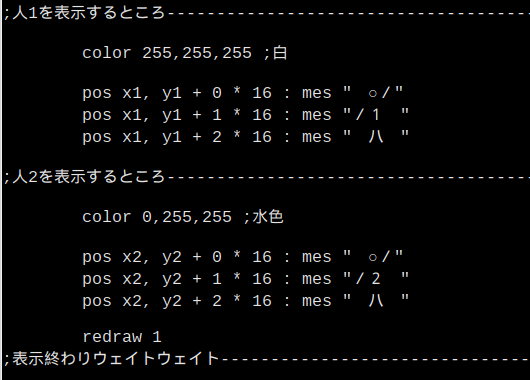
\includegraphics[keepaspectratio,width=12.326cm,height=8.123cm]{text04-img/text04-img007.png}
\flushleft

Figure \stepcounter{Figure}{\theFigure}: ミニサッカーゲームのプログラム}
\end{minipage}

\bigskip
\bigskip
\bigskip

プログラムから、mes命令で人を表示している部分を探して改造してみましょう。

mes命令は、

\bigskip

{\bfseries
mes \ “文字”}


\bigskip

のように必ず「”」の記号で文字を囲む必要があるので忘れないでください。

\bigskip
\bigskip

{\bfseries
例題1 答え}


\bigskip

[F5]キーを押して改造した人がきちんと表示されるかどうか確認しましょう。

\ \ \ \ 人を改造することで、見た目が変わってあなただけのゲームに変わります。

改造ができたらTAや周りの友達にも見せてあげましょう。


\bigskip




\clearpage
{\bfseries
[重要]エラーが出て動かなくなった時は}

\bigskip

プログラムを改造していると、[F5]キーを押して実行しようとしても、エラーが発生して動かなくなったり、絵がおかしくなったりすることがあります。

\bigskip

\bigskip
\bigskip

\begin{minipage}{9.781cm}
\centering
{\upshape
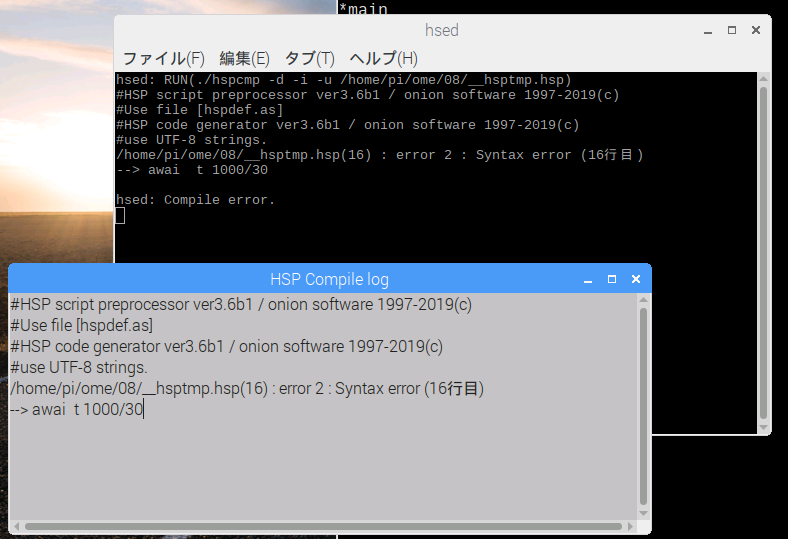
\includegraphics[keepaspectratio,width=11.324cm,height=7.756cm]{text04-img/text04-img011.png}
\flushleft

Figure \stepcounter{Figure}{\theFigure}: エラーの表示}
\end{minipage}

\bigskip
\bigskip
\bigskip

エラーが発生した時は、エラーの内容と「(xx行目)」というエラーの場所が示されます。

エディタの左下に現在カーソルがある行番号が表示されているので、エラーの場所を見直してください。

わからない時は、先生かTAに質問してみましょう。

どうしても動かなくなってしまった時には、元になっているファイルが保存されているので、

「/usr/local/share/ome/04」フォルダ内の元のファイル(kick.hsp)をもう一度コピーして使ってみてください。




\clearpage
\subsection{例題4-2 ミニサッカーゲームのボールや色を変える}
\bigskip
\bigskip

{\bfseries
考え方}

\bigskip

\bigskip

ミニサッカーゲーム(kick.hsp)のプログラムを改造してゲームの内容を変えてみましょう。

\bigskip

ゲームの中に出てくるサッカーボールもmes命令によって表示されています。

\bigskip
\bigskip

\begin{minipage}{9.781cm}
\centering
{\upshape
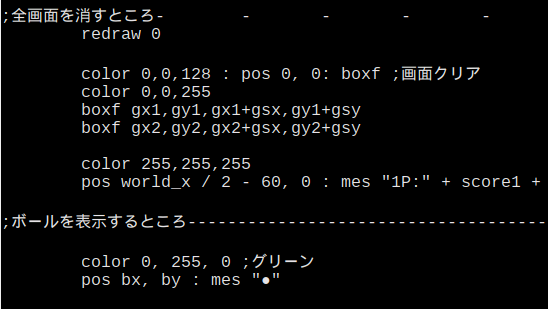
\includegraphics[keepaspectratio,width=14.499cm,height=2.91cm]{text04-img/text04-img008.png}
\flushleft

Figure \stepcounter{Figure}{\theFigure}: ミニサッカーゲームのプログラム}
\end{minipage}

\bigskip
\bigskip
\bigskip

このボールも変えることができます。

プログラムの中から、ボールを出している部分を探して変更しましょう。


\bigskip

color命令は、色を決める命令だということを覚えていますか?

第2回で覚えたcolor命令の使い方を思い出しながら、ボールの色を変えてみましょう。

\bigskip
\bigskip

\begin{minipage}{9.781cm}
\centering
{\upshape
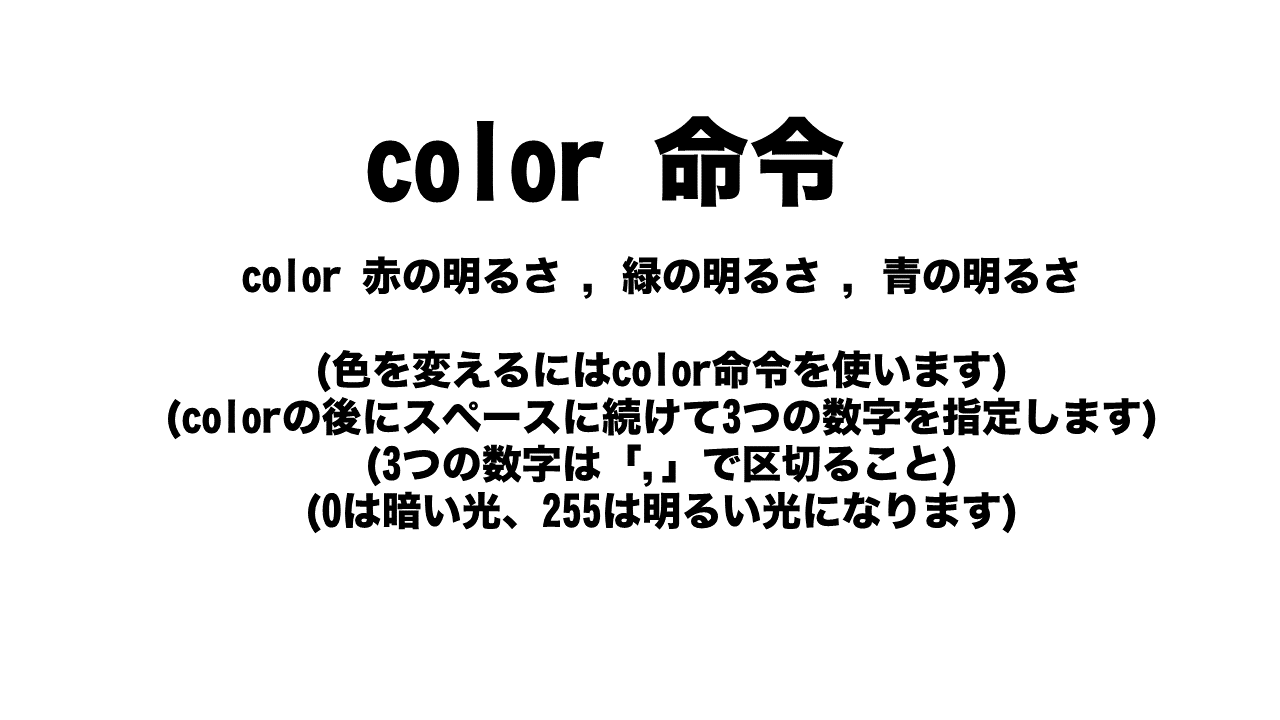
\includegraphics[keepaspectratio,width=12.409cm,height=7.62cm]{text04-img/text04-img009.png}}
\end{minipage}

\bigskip
\bigskip
\bigskip

このゲームでは画像を一切使っていません。

背景のゴール、人、ボールも含めてすべてプログラムの中で決めています。

boxf命令は、好きな大きさの四角形を画面に出すことのできる命令です。

この命令とcolorを組み合わせて背景となる色やゴールを出しています。

\bigskip

実際に色を書き換えて、オリジナルのサッカーゲームを作ってみましょう。

タイトルの文字や、得点を表示する文字も変えることができます。

\bigskip

\bigskip

{\bfseries
例題4-2 答え}

\bigskip

[F5]キーを押して改造した部分がきちんと表示されるかどうか確認しましょう。

\ \ \ \ プログラムを改造することで、見た目が変わってあなただけのゲームに変わります。

改造ができたらTAや周りの友達にも見せてあげましょう。

\bigskip

\bigskip

\clearpage
\subsection{例題4-3 ミニサッカーゲームの動きを改造する}
\bigskip
\bigskip

{\bfseries
考え方}

\bigskip

\bigskip

ミニサッカーゲーム(kick.hsp)のプログラムを改造してゲームの内容を変えてみましょう。

このプログラムでは、変数を使って人の動きや、ボールの動きを計算しています。

変数の代入と計算の方法を覚えていますか?


\bigskip

プログラムの最初に、変数に値を代入しています。

この値を変更することで、ゲームの動きが大きく変わります。

\bigskip
\bigskip

\begin{minipage}{9.781cm}
\centering
{\upshape
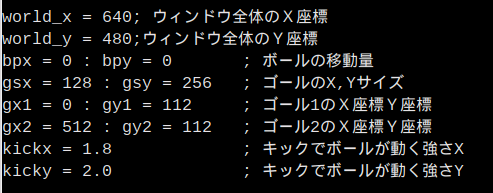
\includegraphics[keepaspectratio,width=13.044cm,height=5.106cm]{text04-img/text04-img010.png}
\flushleft

Figure \stepcounter{Figure}{\theFigure}: ミニサッカーゲームのプログラム}
\end{minipage}

\bigskip
\bigskip
\bigskip

でたらめに書き直してもエラーになったり、処理が遅くなったりするので、あまり大きく変えないようにしましよう。

どの変数が、どのような働きをしているかをコメントとして書いてあります。


\bigskip

{\bfseries
\ \ 変数 = 数字 \ \ \ \ \ \ \ \ \ \ \ \ \ \ \ \ \ \ \ \ \ \ \ \ \ \ \ \ \ \ \ \ \ \ ; コメント}


\bigskip

となっている時、「; コメント」の部分は、プログラムの実行には関係ないですがメモを残す意味で、文字が書かれています。「;」記号から後ろはコメントとして扱われるルールだということを覚えておきましょう。

Xは横方向の動きを表しています。Yは縦方向です。

数字を変えてどのように変わるか試してみましょう。


\bigskip


\bigskip

{\bfseries
例題4-3 答え}


\bigskip

「kickx = 1.8」の数字を少しだけ大きくしてみましょう。

(大きくしすぎないようにしてください)

「kicky = 2.0」なども変えてみると、どうなるか確認してみましょう。


\bigskip

[F5]キーを押して改造したゲームがきちんと動くか確認しましょう。

改造ができたらTAや周りの友達にも見せてあげましょう。


\bigskip




  % Modify:

\clearpage
\section{プログラムと画像ファイルについて知ろう}


\subsection{絵を出してみよう}
\bigskip
\bigskip

ゲームを作る場合には、きれいな絵を出したいですよね。

ここでは、HSPで文字だけでなく、絵を出す方法について学んでいきましょう。

\bigskip

まずは、簡単なプログラムから見てみましょう。

スクリプトエディタの、ファイル→「開く」メニューから「celput.hsp」を読み込んでください。

終わったら、さっそく[F5]キーを押してプログラムを実行してみましょう。

\bigskip
\bigskip

\begin{minipage}{9.781cm}
\centering
{\upshape
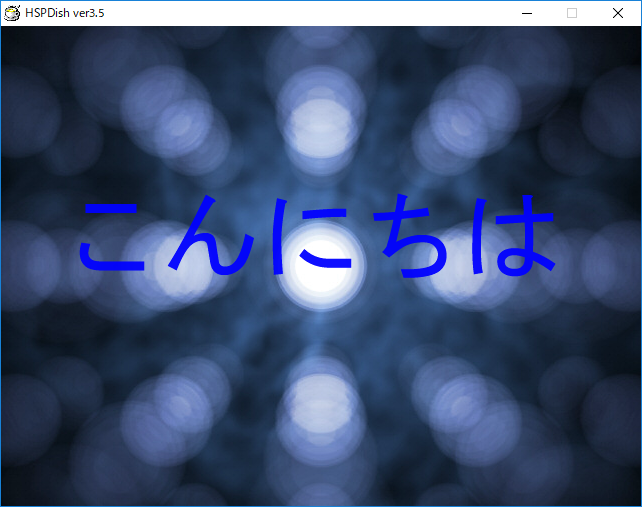
\includegraphics[keepaspectratio,width=10.028cm,height=7.909cm]{text04-img/text04-img012.png}
\flushleft

Figure \stepcounter{Figure}{\theFigure}: celput.hspの実行画面}
\end{minipage}

\bigskip
\bigskip
\bigskip

今度は、背景に絵が出ました。

この絵は、あらかじめ「sozai1.jpg」というファイルで用意されているものです。

実際に絵を出すためには、画像ファイルと呼ばれる絵のデータが必要になります。

それが、「sozai1.jpg」になります。(画像ファイルは、GIMPツールや、ブラウザなどで開くことができます。)


\bigskip

絵を出すためには、2つの命令を使う必要があります。1つ目のcelloadは、最初に必要な絵の素材を知らせるための命令です。これにより、指定された素材を表示する準備をします。


\bigskip

{\bfseries
\ \ celload “画像ファイル名” , 絵の番号\ \ \ \ \texttt{← 絵を出す準備をする}}

\bigskip

一度、celload命令によって登録された絵は、celput命令によって表示させることができます。

celload命令は、最初の1回だけ実行すれば良いです。以降は、celput命令によって、mes命令やboxf命令と同じように絵を出すことができるようになります。


\bigskip

celput命令は、以下のように書くことができます。


\bigskip

{\bfseries
\ \ celput 絵の番号}

\bigskip

絵の番号というのは、celload命令で指定していた番号のことです。

出すための絵を登録する時に、1,2,3,4…というように、別々な番号を割り振っておいて、同時に色々な絵を出せるようにするための仕組みです。

最初は、番号1を使っておきましょう。

\bigskip
\bigskip

\begin{minipage}{9.781cm}
\centering
{\upshape
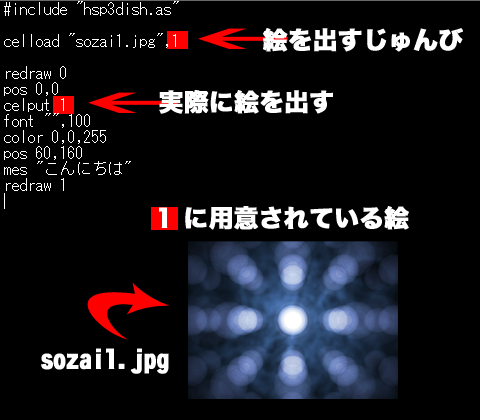
\includegraphics[keepaspectratio,width=12.806cm,height=11.206cm]{text04-img/text04-img013.png}}
\end{minipage}

\bigskip
\bigskip
\bigskip

つまり、

\bigskip

{\bfseries
\ \ celload “sozai1.jpg”,1}

\bigskip

は、番号1で「sozai1.jpg」の絵を表示するための準備をするという意味になります。

celputで指定した番号に準備された絵を表示します。

表示する位置は、mes命令などと同じようにpos命令で指定された位置になります。

準備する画像のファイルは、プログラム(.hsp)がある場所と同じフォルダに入れておく必要があります。

画像ファイル、「sozai1.jpg」は、04フォルダ内にあるはずです。


\bigskip

celload命令とcelput命令、絵を出す番号と画像ファイルの関係をよく覚えておきましょう。

\bigskip
\bigskip
\bigskip

\subsection{例題に挑戦しよう}

\bigskip
\bigskip

終わってしまった人は、以下の例題にも挑戦してみよう。

\bigskip

・色々な絵と文字を表示しよう

・自分で用意した絵を表示する


\bigskip

例題の考え方がわからない時は、近くのTAか先生に聞いてください。

わからない所は、そのままにせず、必ず答えを見つけてから先に進みましょう。

\clearpage
\subsection{例題4-4 色々な絵と文字を表示する}
\bigskip
\bigskip

{\bfseries
考え方}

\bigskip

絵と文字を表示するプログラム(celput.hsp)を改造してみましょう。


\bigskip

{\bfseries
\ \ celload “sozai1.jpg”,1}


\bigskip

は「sozai1.jpg」という画像ファイルを表示するための準備をします。

\bigskip

[資料] 背景として使える画面の一例

   ( sozai1.jpg 〜 sozai20.jpg )

\bigskip
\bigskip

\begin{minipage}{9.781cm}
\centering
{\upshape
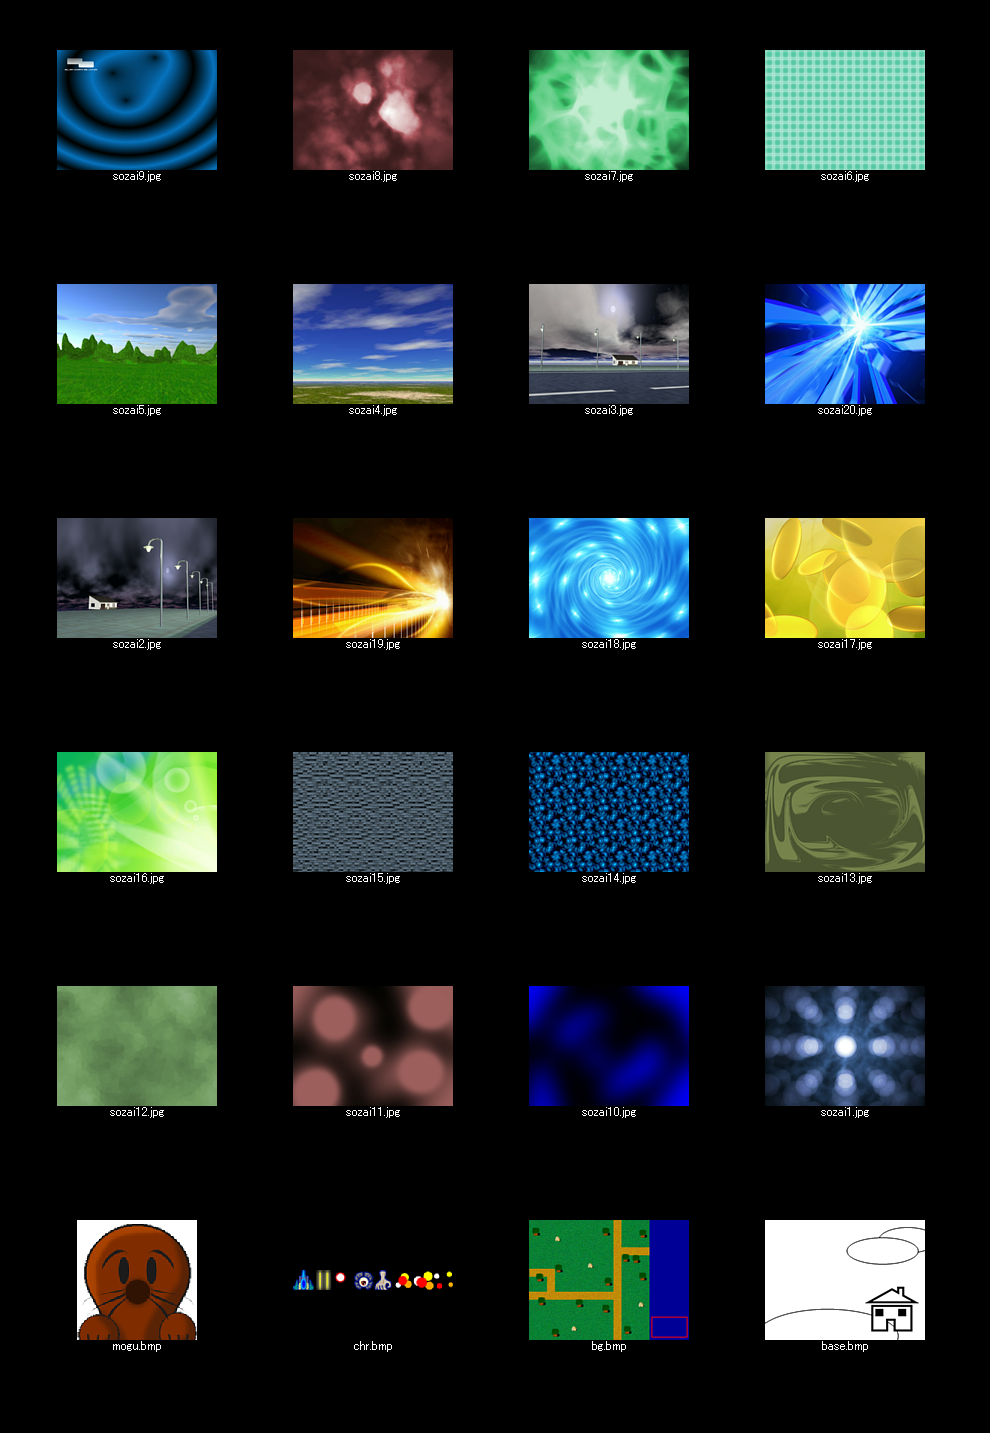
\includegraphics[keepaspectratio,width=14.843cm,height=17.609cm]{text04-img/text04-img014.png}}
\end{minipage}

\bigskip
\bigskip
\bigskip


試しに、celload命令で指定している画像ファイル名を他のものに変更して、実行してみましょう。

このように自由な絵を使って画面を作っていくことができます。

\bigskip

\bigskip


{\bfseries
例題4-4 答え}

\bigskip

「04」フォルダには、自由に使える素材として「sozai1.jpg」から「sozai20.jpg」まで20種類の画像ファイルが含まれています。

[F5]キーを押して改造した画面がきちんと表示されるかどうか確認しましょう。

mes命令、font命令、color命令、pos命令も書き換えることで、違ったメッセージを表示させることができます。

改造ができたらTAや周りの友達にも見せてあげましょう。

\bigskip


\clearpage
\subsection{例題4-5 自分で用意した絵を表示する}
\bigskip
\bigskip

{\bfseries
考え方}

\bigskip

絵と文字を表示するプログラム(celput.hsp)を改造して自分で用意した絵を出してみましょう。

準備する画像のファイルは、プログラム(.hsp)がある場所と同じフォルダに入れておく必要があります。


\bigskip

\ \ celput.hsp

\ \ sozai1.jpg


\bigskip

が同じディレクトリにあることを確認しましょう。

同じように「04」フォルダの中に、皆さんが自分で画像を作ったり、コピーして使用することもできます。


\bigskip


\bigskip


\bigskip


\bigskip

{\bfseries
例題4-5 答え}


\bigskip

[F5]キーを押して正しい画像が表示されるかどうか確認しましょう。

改造ができたらTAや周りの友達にも見せてあげましょう。


\bigskip

プログラムをあまり改造しすぎると、動かなくなったり、パソコンの動きが遅くなってしまうことがあります。その時は、先生に聞くか、元のファイル(celput.hsp)をもう一度コピーして使ってみてください。


\bigskip

\bigskip

\clearpage
\subsection{絵を重ねて表示してみよう}
\bigskip
\bigskip

もう少し別な絵を表示してみましょう。

スクリプトエディタの、ファイル→「開く」メニューから「apple.hsp」を読み込んで実行してみてください。

\bigskip
\bigskip

\begin{minipage}{9.781cm}
\centering
{\upshape
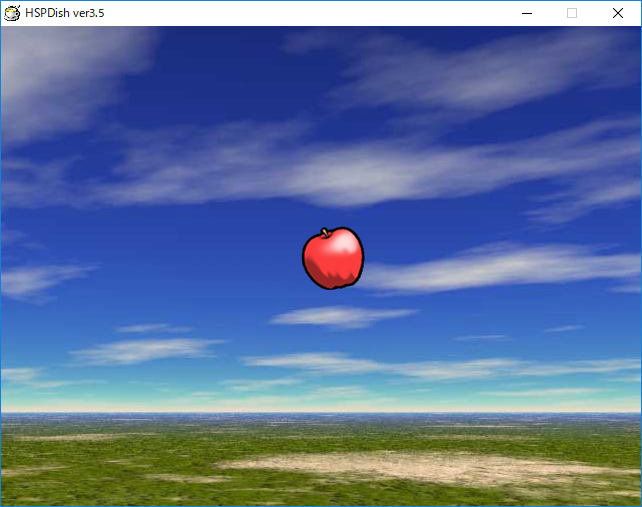
\includegraphics[keepaspectratio,width=9.634cm,height=7.599cm]{text04-img/text04-img015.png}
\flushleft

Figure \stepcounter{Figure}{\theFigure}: apple.hspの実行画面}
\end{minipage}

\bigskip
\bigskip
\bigskip

今度は、画面の中央に「りんご」が表示されていることに気付いたでしょうか。


\bigskip

実は、このプログラムでは背景と「りんご」の2つの画像を使っています。

背景の上に「りんご」を表示しているのです。

\bigskip
\bigskip

\begin{minipage}{9.781cm}
\centering
{\upshape

\includegraphics[keepaspectratio,width=2.249cm,height=2.249cm]{text04-img/text04-img016.png}
\flushleft

Figure \stepcounter{Figure}{\theFigure}: リンゴの画像( apple.png )}
\end{minipage}

\bigskip
\bigskip
\bigskip

\bigskip
\bigskip

\begin{minipage}{9.781cm}
\centering
{\upshape
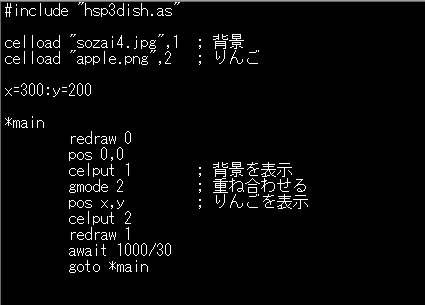
\includegraphics[keepaspectratio,width=11.245cm,height=8.07cm]{text04-img/text04-img017.png}}
\end{minipage}

\bigskip
\bigskip
\bigskip

このように複数の番号を登録して、celput命令を使うことで絵を重ねて表示することができます。

そのために、gmodeという新しい命令が使われています。


\bigskip

{\bfseries
\ \ (HSPのルール)}

\bigskip

{\bfseries
\ \ 画像を重ねる設定をするにはgmode命令を使います

\ \ gmodeの後、スペースに続けてコピーモードを示す数字を指定します

\ \ コピーモードは、以下のような意味があります

\ \ \ \ 0のとき \ \ \ \ \ \ \ : 画像のまま表示

\ \ \ \ 1か2のとき \ \ \ : 透明な部分は背景を残して表示

\ \ \ \ 3のとき \ \ \ \ \ \ \ : 透明度を変えて表示}

\bigskip

「gmode 2」を指定することで、リンゴの透明な部分は背景が表示されて、きれいに重なっているように見えています。試しに、「gmode 0」にしてリンゴの絵がどのように表示されるか確認してみましょう。

リンゴのように透明な部分がある絵は、以前にも使ったGIMPツールで作ったり、確認することができます。GIMPは、画像ファイルの右クリックメニューから「GNU Image Manipulation Program」を選択することで起動させることができます。

\bigskip
\bigskip

\begin{minipage}{9.781cm}
\centering
{\upshape
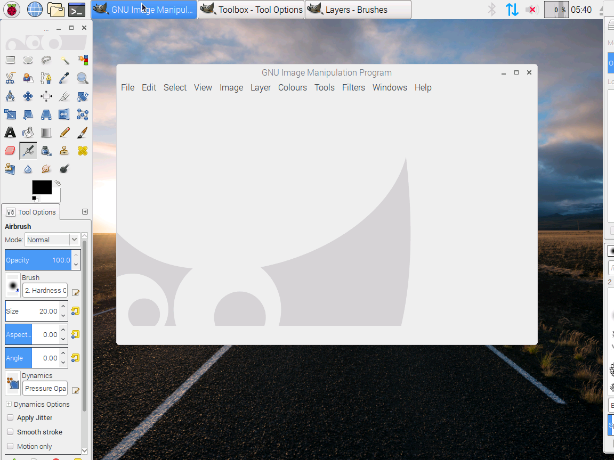
\includegraphics[keepaspectratio,width=7.091cm,height=5.318cm]{text04-img/text04-img018.png}
\flushleft

Figure \stepcounter{Figure}{\theFigure}: GIMPを起動した画面}
\end{minipage}

\bigskip
\bigskip
\bigskip

celput命令には、実はもっと多くのパラメーターがあります。


\bigskip

{\bfseries
\ \ celput 絵の番号, 分割画像No. , 横方向の表示倍率, 縦方向の表示倍率, 回転角度}

\bigskip

{\bfseries
横方向の表示倍率=0.0〜(1.0) : 横方向の表示倍率(実数)

縦方向の表示倍率=0.0〜(1.0) : 縦方向の表示倍率(実数)

回転角度=0.0〜(0.0) : 回転角度(実数)}

\bigskip

絵を自由な大きさ、角度で出すことができるようになっています。

通常は、倍率1、角度0の状態で表示されます。

分割画像No.は、1つの画像を複数の小さなブロックに分けて表示するための機能です。

(これについては、また別の機会に説明します。)


\bigskip

試しに、表示倍率や角度を変えてみて、どのように表示が変わるか確認してみましょう。

また、余裕がある人は、文字を重ねてさらに複雑な画面を作ることに挑戦してください。


\bigskip

\bigskip

\clearpage
\subsection{絵を動かしてみよう}
\bigskip
\bigskip

今度は、表示した絵を動かしてみることにしましょう。

絵が動くことで、ゲームやアニメーションなどさらに応用が広がります。

そのために覚えておかなければならないのが、変数です。


\bigskip

変数について学んだことを覚えていますか?


\bigskip

{\bfseries
\ \ (HSPのルール)

\bigskip

\ \ 「変数の名前=数値」で変数に値を入れることができる(代入)

\ \ 変数に数値を入れておくとパラメーターとして使える

\ \ mes命令の中で「+変数」を書くことで変数の中身を表示できる}


\bigskip

「a=100」と置くと、変数aに100という数字が記憶されます。

これを使って、いままで数字を書いていた部分に変数を代わりに書いて数字を変化させることができます。


\bigskip

スクリプトエディタの、ファイル→「開く」メニューから「fall.hsp」を読み込んで実行してみてください。

\bigskip
\bigskip

\begin{minipage}{9.781cm}
\centering
{\upshape
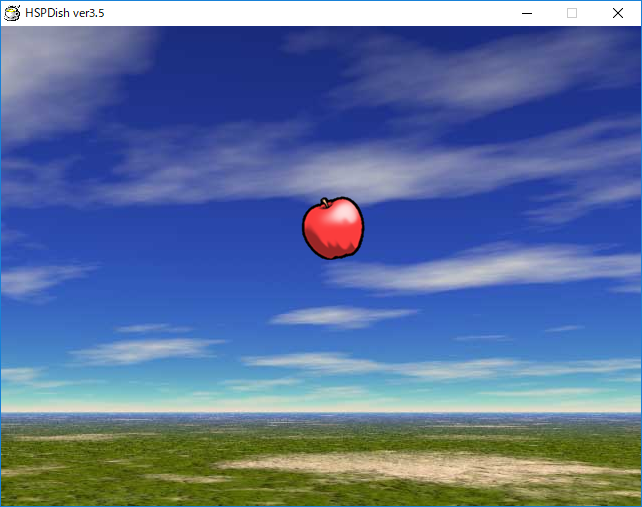
\includegraphics[keepaspectratio,width=9.183cm,height=7.241cm]{text04-img/text04-img019.png}
\flushleft

Figure \stepcounter{Figure}{\theFigure}: fall.hspの実行画面}
\end{minipage}

\bigskip
\bigskip
\bigskip

今度はリンゴが動いているのがわかると思います。

\bigskip
\bigskip

\begin{minipage}{9.781cm}
\centering
{\upshape
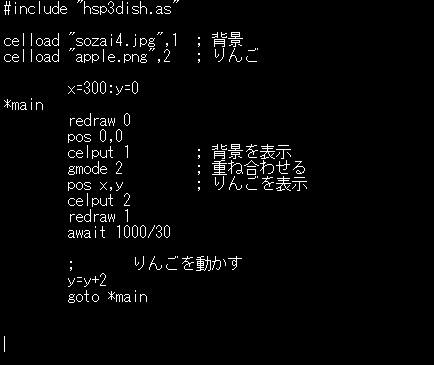
\includegraphics[keepaspectratio,width=10.954cm,height=9.213cm]{text04-img/text04-img020.png}}
\end{minipage}

\bigskip
\bigskip
\bigskip

プログラムを見てみましょう。

\bigskip

変数xと変数yが、リンゴの横、縦の位置を記憶しています。

最初に「x=300:y=0」の行で、変数xに300を、変数yに0を代入しています。


\bigskip

{\bfseries
\ \ (HSPのルール)

\bigskip

「:」の記号を入れると、行を分けたのと同じように別な命令を書ける

\ \ 「:」の記号を使って1行にたくさんの命令を書くことができる}


\bigskip

「pos x,y」がありますので、celputする時の位置を変数x,yで変えられるようになっています。

つまり、横の位置が変数x、縦の位置が変数yに記憶されていることになります。


\bigskip

実際にリンゴの位置を変えているのが、「y=y+2」の部分です。

ここを繰り返し実行することで、変数yの値が2ずつ増えていきます。


\bigskip

{\bfseries
\ \ (HSPのルール)

\bigskip

\ \ 数式とは、数値と変数、またはそれらを計算式でつなげて書くこと

\ \ 「+」は足し算、「-」は引き算、「*」は掛け算(×)、「/」は割り算(÷) }


\bigskip

「y=y+2」は変数yに記憶されている数字に2を足すという意味だと覚えておきましょう。

これで、縦の位置が少しずつ変化するようになります。


\bigskip
\bigskip
\bigskip

\subsection{例題に挑戦しよう}

\bigskip
\bigskip

終わってしまった人は、以下の例題にも挑戦してみよう。

\bigskip

・色々な動きに挑戦してみよう

・自分で用意した絵を動かして表示する


\bigskip

例題の考え方がわからない時は、近くのTAか先生に聞いてください。

わからない所は、そのままにせず、必ず答えを見つけてから先に進みましょう。

\clearpage
\subsection{例題4-6 色々な動きに挑戦してみよう}
\bigskip
\bigskip

{\bfseries
考え方}

\bigskip

りんごを動かすプログラム(apple.hsp)を改造して動きを変えてみましょう。

\bigskip
\bigskip

\begin{minipage}{9.781cm}
\centering
{\upshape
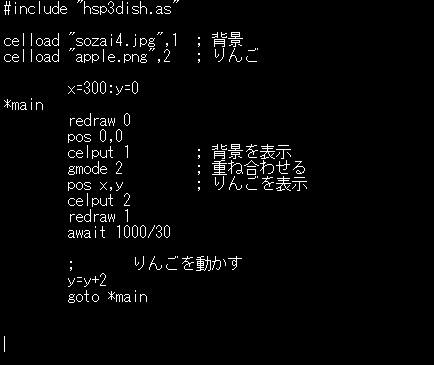
\includegraphics[keepaspectratio,width=10.954cm,height=9.213cm]{text04-img/text04-img020.png}}
\end{minipage}

\bigskip
\bigskip
\bigskip

変数xとyが、横と縦の位置を記憶していることはわかりましたか。

「y=y+2」という計算で下に向かって絵が動いていきます。

もっと速く動かすにはどうすればいいでしょうか?

別な方向、たとえば左から右、下から上に動かす方法を考えてみましょう。


\bigskip


\bigskip


\bigskip

{\bfseries
例題4-6 答え}


\bigskip

変数xの値を計算で変えることで横方向に、変数yの値を計算で変えることで縦方向に動かすことができます。

たとえば、「x=x+2」は右に、「y=y-2」は上に動くことになります。

計算で使っている「2」という数字は、1つのコマで動く大きさになります。

この値を変えることで、動く速さも変わります。大きな数字で速い速度、小さな数字で遅くなることを確認してみましょう。

\clearpage
\subsection{例題4-7 自分で用意した絵を動かして表示する}
\bigskip
\bigskip

{\bfseries
考え方}

\bigskip

apple.hspのプログラムを使って、自分で作った絵を動かすようにしてみましょう。

表示させるための画像は、GIMPツールで作ったり、確認することができます。GIMPは、Raspberry
Piメニューからグラフィックス→「GNU Image Manipulation Program」をクリックすることで起動させることができます。

りんごの画像は、「apple.png」です。

開くメニューから、「apple.png」を読み込んで編集してください。

背景にあたる部分は、消しゴムで消す必要があるので注意してください。

\bigskip
\bigskip

\begin{minipage}{9.781cm}
\centering
{\upshape
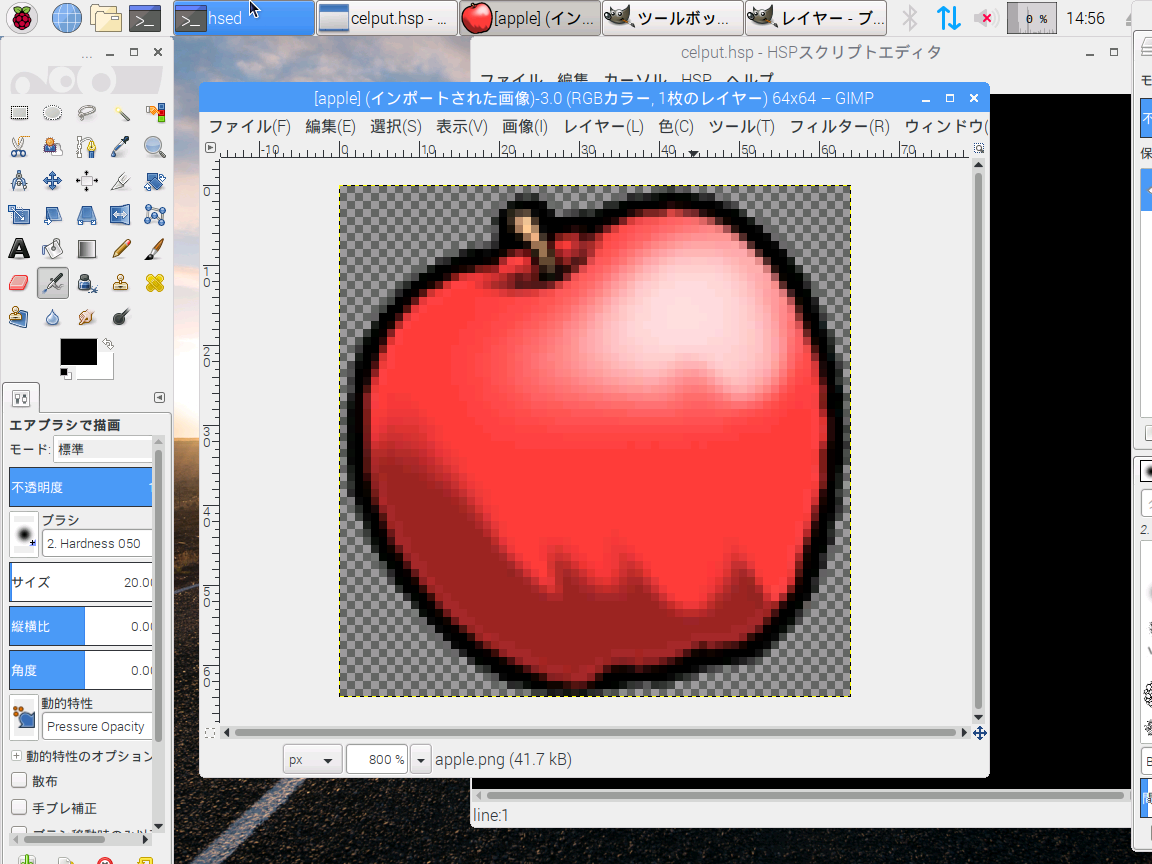
\includegraphics[keepaspectratio,width=11.712cm,height=8.784cm]{text04-img/text04-img021.png}
\flushleft

Figure \stepcounter{Figure}{\theFigure}: GIMPの編集画面}
\end{minipage}

\bigskip
\bigskip
\bigskip

\bigskip

{\bfseries
例題4-7 答え}


\bigskip

GIMPで修正できたら、[F5]キーを押して改造した人がきちんと表示されるかどうか確認しましょう。

自分で別な画像ファイルを用意した場合は、


\bigskip

{\bfseries
\ \ celload “apple.png”,2}

\bigskip

のファイル名を修正してください。

元のりんご画像に戻したい時は、元のファイル(apple.png)をもう一度コピーして使ってみてください。

\bigskip


  % Jump Action:

\clearpage
\section{ジャンプアクションゲームに挑戦しよう}


\subsection{ジャンプアクションゲームのあそびかた}
\bigskip
\bigskip

ジャンプアップゲームでキャラクターを動かして遊ぶ本格的なゲームを体験してみましょう。


\bigskip

ファイル→「開く」メニューから「jump.hsp」を読み込んでください。

見つからない場合は、まわりの友達か、近くの先生に聞いてみてください。

\bigskip

[F5]キーで実行すると、タイトル画面が出ます。[Enter]キーを押して始めてください。

\bigskip
\bigskip

\begin{minipage}{9.781cm}
\centering
{\upshape
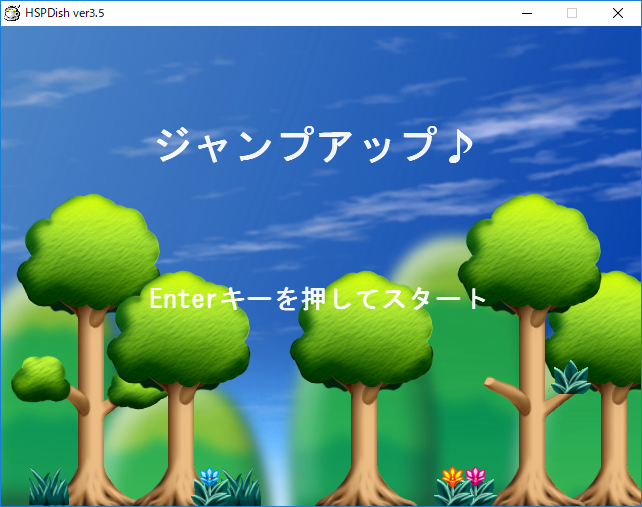
\includegraphics[keepaspectratio,width=11.192cm,height=8.827cm]{text04-img/text04-img022.png}
\flushleft

Figure \stepcounter{Figure}{\theFigure}: タイトル画面}
\end{minipage}

\bigskip
\bigskip
\bigskip

ジャンプアップゲームは、キャラクターを操作してコインを取るゲームです。

左右の移動とジャンプをさせることができます。

\bigskip
\bigskip

\begin{minipage}{9.781cm}
\centering
{\upshape
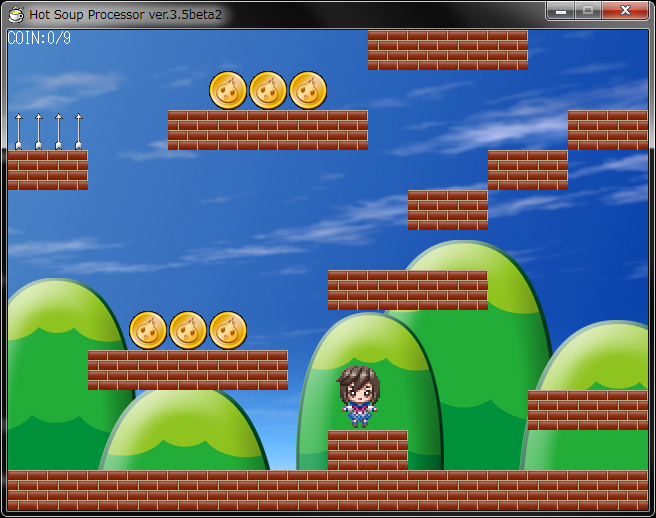
\includegraphics[keepaspectratio,width=11.28cm,height=8.915cm]{text04-img/text04-img023.png}
\flushleft

Figure \stepcounter{Figure}{\theFigure}: ジャンプアップゲーム画面}
\end{minipage}

\bigskip
\bigskip
\bigskip

矢印のキーで左右に動かして、スペースキーでジャンプです。

ジャンプしながら、コインを取って上に進みましょう。

すべてのコインを取るとあなたの勝ちです。逆に、地面に置かれている矢に当たってしまうとゲームオーバーになってしまいます。

\bigskip
\bigskip

\begin{minipage}{9.781cm}
\centering
{\upshape
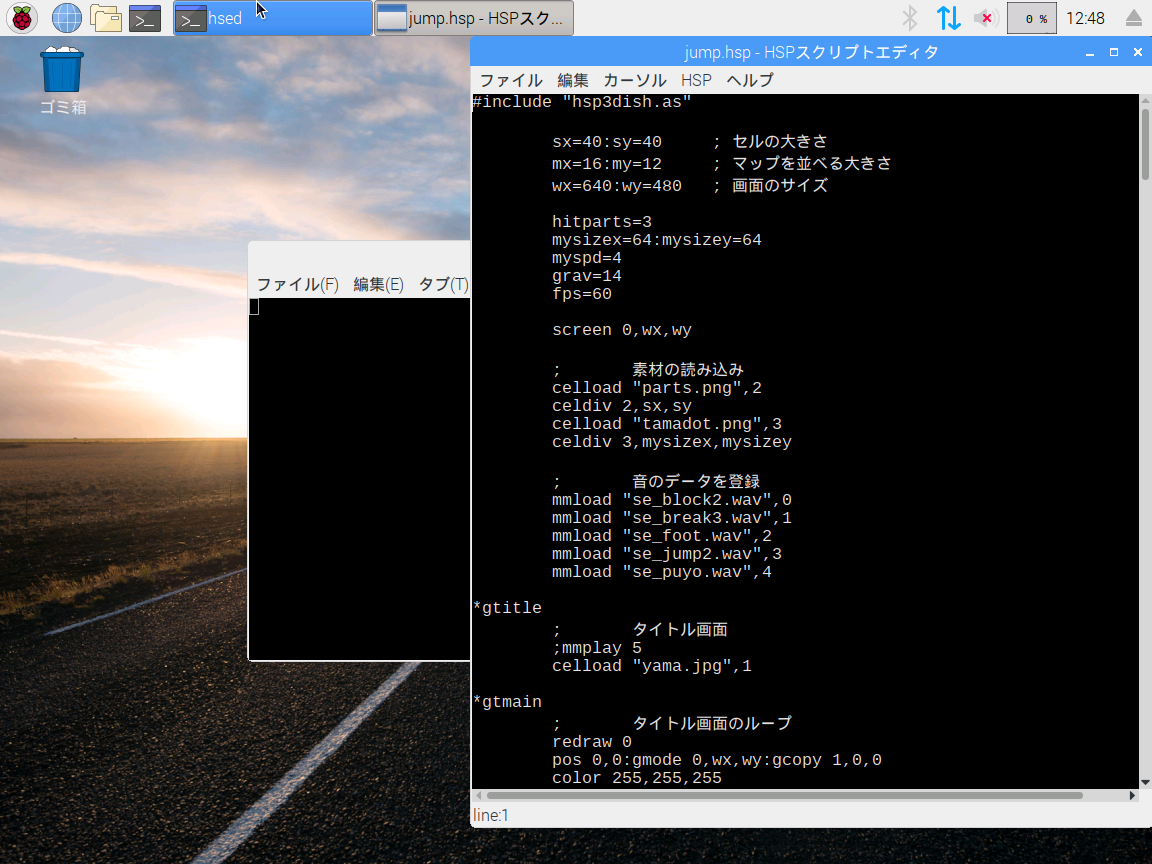
\includegraphics[keepaspectratio,width=11.192cm,height=8.393cm]{text04-img/text04-img024.png}
\flushleft

Figure \stepcounter{Figure}{\theFigure}: ジャンプアップゲームのプログラム}
\end{minipage}

\bigskip
\bigskip
\bigskip

\subsection{例題に挑戦しよう}

\bigskip
\bigskip

ゲームが遊べた人は、以下の例題にも挑戦してみよう。

\bigskip

・オリジナルの面を作ってみよう

・ゲームの動きを改造してみよう

・ゲームの背景や絵を改造してみよう

・ゲームのタイトル画面を改造してみよう


\bigskip

例題の考え方がわからない時は、近くのTAか先生に聞いてください。

わからない所は、そのままにせず、必ず答えを見つけてから先に進みましょう。

\clearpage
\subsection{例題4-8 オリジナルの面を作ってみよう}
\bigskip
\bigskip

{\bfseries
考え方}

\bigskip

ジャンプアップゲーム(jump.hsp)のプログラムを改造してゲームで使われている面(マップ)を変えてみましょう。

プログラムを編集することで、面のデータを自分で変えることができます。

以下の場所を探して編集します。

\bigskip
\bigskip

\begin{minipage}{9.781cm}
\centering
{\upshape
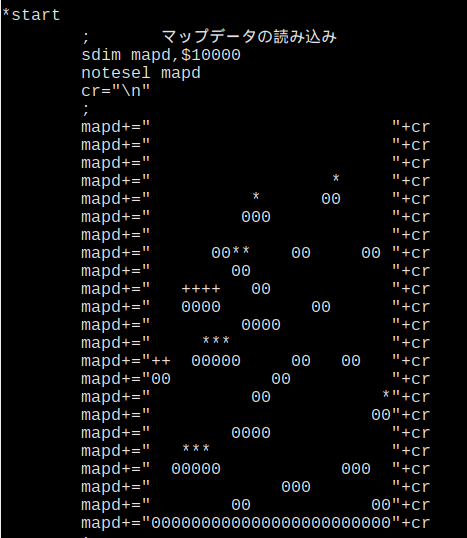
\includegraphics[keepaspectratio,width=10.478cm,height=12.07cm]{text04-img/text04-img025.png}}
\end{minipage}

\bigskip
\bigskip
\bigskip

{\bfseries
\ \ 「0」はレンガ(壁)になります。

\ \ 「*」はコイン、「+」は矢になります。

\ \ マップデータが書かれている場所を探して、自分だけの面を作ってみましょう。}


\bigskip

でたらめに書き直してもエラーが出るだけです。必ず、


\bigskip

{\bfseries
\ \ mapd+=” \ \ \ \ \ \ \ \ \ \ \ \ \ \ \ \ \ \ \ \ \ \ \ \ \ \ \ \ “+cr}


\bigskip

という形になるようにしてください。

文字は「”」で囲み、最後に「+cr」を入れます。

面のデータは、縦・横方向に広げることができます。


\bigskip


\bigskip

{\bfseries
例題4-8 答え}


\bigskip

ゲームを改造することで、難しくなったり、簡単になったりします。

改造ができたらTAや周りの友達にも見せてあげましょう。


\clearpage
\subsection{例題4-9 ゲームの動きを改造してみよう}
\bigskip
\bigskip

{\bfseries
考え方}

\bigskip

ジャンプアップゲーム(jump.hsp)のプログラムは、最初にゲームの動きを決める変数が決められた数字で代入されています。

慣れてきたら、改造できる部分を自分で探してみましょう。

\bigskip
\bigskip

\begin{minipage}{9.781cm}
\centering
{\upshape
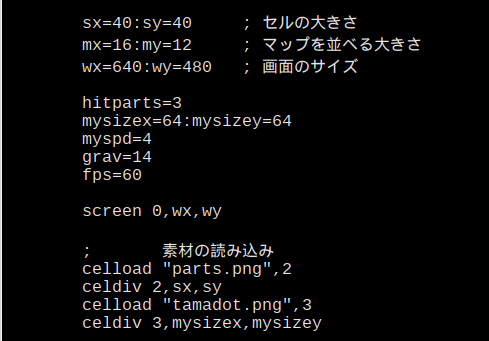
\includegraphics[keepaspectratio,width=11.853cm,height=8.266cm]{text04-img/text04-img026.png}}
\end{minipage}

\bigskip
\bigskip
\bigskip

「セルの大きさ」「マップを並べる大きさ」「画面のサイズ」はそのままにしておいてください。

mypd、gravといった変数の値を変えるとどうなるか、試してみましょう。


\bigskip


\bigskip


\bigskip


\bigskip

{\bfseries
例題4-9 答え}


\bigskip

「myspd=4」が歩くスピードを決めています

「grav=14」がジャンプの強さを決めています


\bigskip

動きが変わったら、どんな値だと良いバランスのゲームになるか考えてみましょう。

改造ができたらTAや周りの友達にも見せてあげましょう。


\clearpage
\subsection{例題4-10 ゲームの背景や絵を改造してみよう}
\bigskip
\bigskip

{\bfseries
考え方}

\bigskip

ジャンプアップゲーム(jump.hsp)のプログラムで使われている画像を確認してみましょう。

画像を書き換えて、自分だけのゲーム画面を作ることもできます。

\bigskip
\bigskip

\begin{minipage}{9.781cm}
\centering
{\upshape
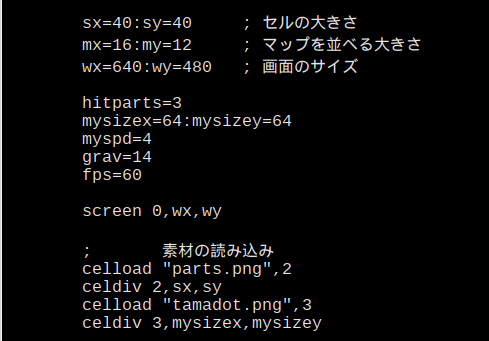
\includegraphics[keepaspectratio]{text04-img/text04-img026.png}}
\end{minipage}

\bigskip
\bigskip
\bigskip

celload命令で読み込まれているファイルが、ゲームに出てくる画像となります。

操作する主人公は「tamadot.png」という画像です

面を構成するパーツは、「parts.png」という画像にまとめられています。

\bigskip
\bigskip

\begin{minipage}{9.781cm}
\centering
{\upshape
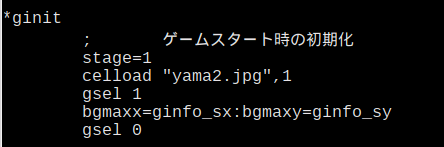
\includegraphics[keepaspectratio,width=10.689cm,height=3.538cm]{text04-img/text04-img027.png}}
\end{minipage}

\bigskip
\bigskip
\bigskip

また、ゲームの背景は、「yama2.jpg」という画像が使われています。

それぞれが、どんな役割を果たしているか、実際にGIMPなどのツールで確認してみましょう。


\bigskip


\bigskip

{\bfseries
例題4-10 答え}


\bigskip

ジャンプアップゲームの背景は、実は小さな絵を並べて、大きな世界を作っています。

GIMPを使って、ジャンプアップゲームの絵を改造してみましょう。

小さな絵を実際に見て改造をしてみましょう。以前にやった手順を覚えていますか?

「parts.png」アイコンの右クリックメニューから「GNU Image Manipulation Program」をクリックして、GIMPツールを起動させましょう。

\bigskip
\bigskip

\begin{minipage}{9.781cm}
\centering
{\upshape
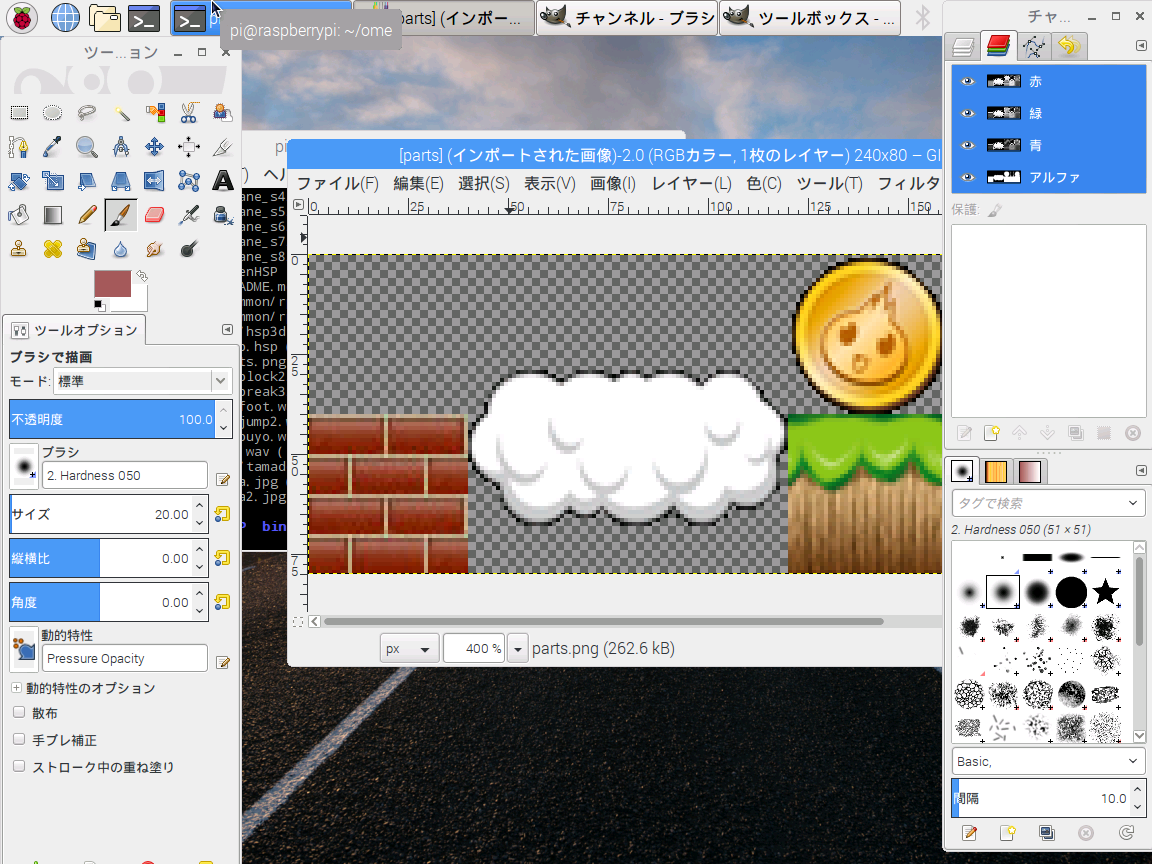
\includegraphics[keepaspectratio,width=12.065cm,height=9.049cm]{text04-img/text04-img029.png}
\flushleft

Figure \stepcounter{Figure}{\theFigure}: parts.pngを修正している画面}
\end{minipage}

\bigskip
\bigskip
\bigskip

パレットで色を選んで、鉛筆のツールで絵を書いていきます。

\bigskip
\bigskip

\begin{minipage}{9.781cm}
\centering
{\upshape
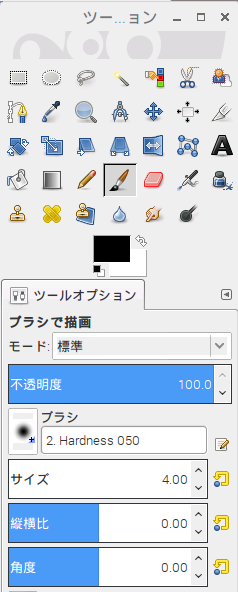
\includegraphics[keepaspectratio,width=4.075cm,height=10.16cm]{text04-img/text04-img030.png}}
\end{minipage}

\bigskip
\bigskip
\bigskip

元の絵があった部分を書き換えて他の絵柄にしてみましょう。


\bigskip

画像が小さい場合は、画像の下にある「100\%」の右側にあるボタンを押して、「400\%」「800\%」などを選ぶと拡大されます。

絵を修正する時には、ツールアイコンの中から「ブラシ」を選択して、サイズを4〜6くらいの数字に変えてから絵の上で、マウスボタンを押しながら動かして色を置きます。


\bigskip

色を変更する場合は、ツールパレットの描画色をクリックして、「描画色の変更」ダイアログを出してから好きな色を選びます。

\bigskip
\bigskip

\begin{minipage}{9.781cm}
\centering
{\upshape
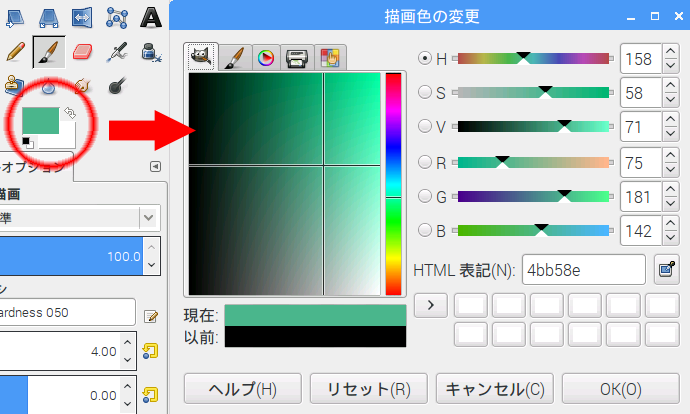
\includegraphics[keepaspectratio,width=10.993cm,height=6.588cm]{text04-img/text04-img031.png}}
\end{minipage}

\bigskip
\bigskip
\bigskip

元の絵を書き換えたら、ファイル→「parts.pngに上書きエクスポート」を選んで保存します。

\bigskip

背景画像は、縦長のもので「yama2.jpg」として保存されています。変更した画像でゲームを動かしてみましょう。

\bigskip
\bigskip

\begin{minipage}{9.781cm}
\centering
{\upshape

\includegraphics[keepaspectratio,width=8.546cm,height=12.804cm]{text04-img/text04-img032.jpg}}
\end{minipage}

\bigskip
\bigskip
\bigskip


[F5]キーを押して実行して変わっていれば成功です。

\bigskip

改造ができたらTAや周りの友達にも見せてあげましょう。

\bigskip


\clearpage
\subsection{例題4-11 ゲームのタイトル画面を改造してみよう}
\bigskip
\bigskip

{\bfseries
考え方}

\bigskip

ジャンプアップゲーム(jump.hsp)のプログラムを改造して、タイトル画面を自分だけのものにしてみましょう。

\bigskip
\bigskip

\begin{minipage}{9.781cm}
\centering
{\upshape
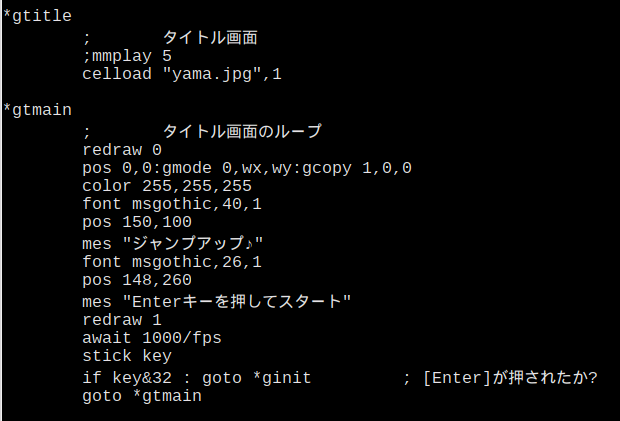
\includegraphics[keepaspectratio,width=14.42cm,height=9.791cm]{text04-img/text04-img033.png}}
\end{minipage}

\bigskip
\bigskip
\bigskip


{\bfseries
例題4-11 答え}


\bigskip

背景の画像に「yama.jpg」、後は決められたサイズと色で文字を出しています。

「ジャンプアップ」ではない、別なタイトルを考えてみましょう。

どんな画面にしたいか、考えてから改造を始めましょう。

\bigskip

改造ができたらTAや周りの友達にも見せてあげましょう。



  % Last Part:

\clearpage
\section{プログラミングの応用}


\subsection{サンプルフォルダを準備しよう}
\bigskip
\bigskip

上にあるバーのアイコンからファイルマネージャーを開いてみましょう。

\bigskip
\bigskip

\begin{minipage}{9.781cm}
\centering
{\upshape
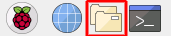
\includegraphics[keepaspectratio,width=5.898cm,height=1.242cm]{text04-img/text02-img001.png}
\flushleft

Figure \stepcounter{Figure}{\theFigure}: ファイルマネージャーを開くアイコン}
\end{minipage}

\bigskip
\bigskip
\bigskip

これからHSPで使うことのできるサンプルプログラムをコピーしてもらいます。「/home/ユーザー名」のフォルダに、「sample」フォルダをコピーすることから始めます。

まず、「/usr/local/share/OpenHSP」という場所を開いてみましょう。

この中に、「sample」という名前のフォルダがあります。これから、この「sample」というフォルダを自分の作業フォルダにコピーします。

「sample」という名前のフォルダ上でマウスの右クリックを押して「コピー」を選んでください。

\bigskip
\bigskip

\begin{minipage}{9.781cm}
\centering
{\upshape
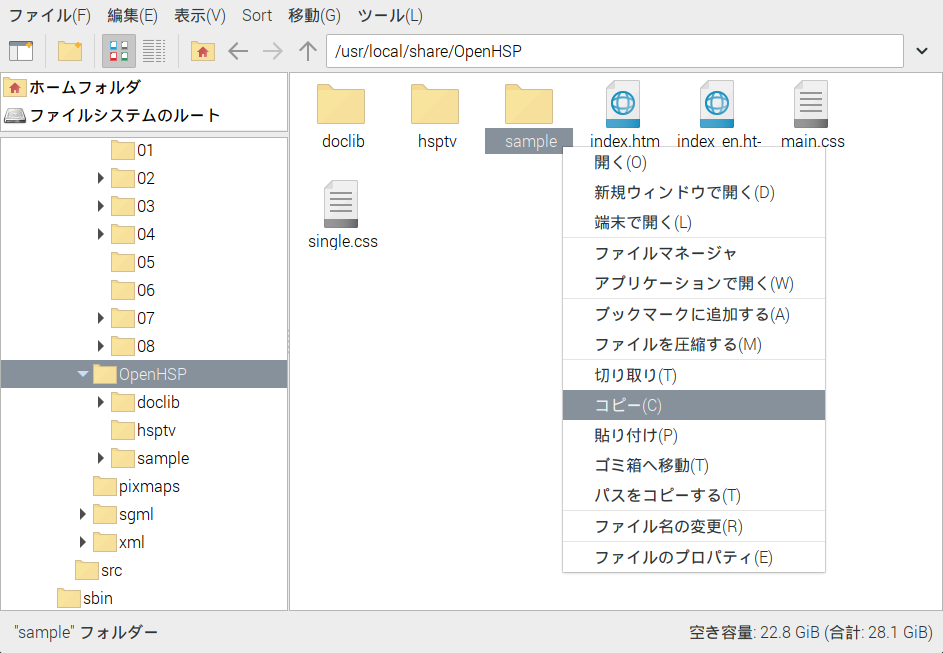
\includegraphics[keepaspectratio,width=11.232cm,height=8.424cm]{text04-img/s_ome04e.png}
\flushleft

Figure \stepcounter{Figure}{\theFigure}: sampleフォルダでコピーを選ぶところ}
\end{minipage}

\bigskip
\bigskip
\bigskip

この後、コピーしたい場所を選びます。コピー先の場所は、「/home/ユーザー名」のフォルダになります。

コピー先の場所を開いたら、何もない場所でマウスの右クリックを押して「貼り付け」を選んでください。

これで先ほどの「/usr/local/share/OpenHSP/sample」フォルダが、「/home/ユーザー名/sample」にコピーされます。

ファイルには、さまざまなプログラムとデータが入っています。

すべてのファイルを紹介できませんが、興味がある人は時間がある時に実際に読み込んで動かしてみましょう。

\bigskip




\clearpage
\subsection{立体的な絵を出すには}
\bigskip
\bigskip

いままで平面的な絵を使ってきました。いわゆる「2D」と呼ばれる表現です。

ゲームやCGでは、立体的な「3D」表現が使われています。実際に、立体的な絵を出すプログラムを動かしてみましょう。


\bigskip

先ほどコピーした「/home/ユーザー名/sample」フォルダの中からプログラムを読み込みます。

ファイル→「開く」メニューから「/home/ユーザー名/sample/hgimg4」内の「light\_test3.hsp」を読み込んでください。

\bigskip
\bigskip

\begin{minipage}{9.781cm}
\centering
{\upshape
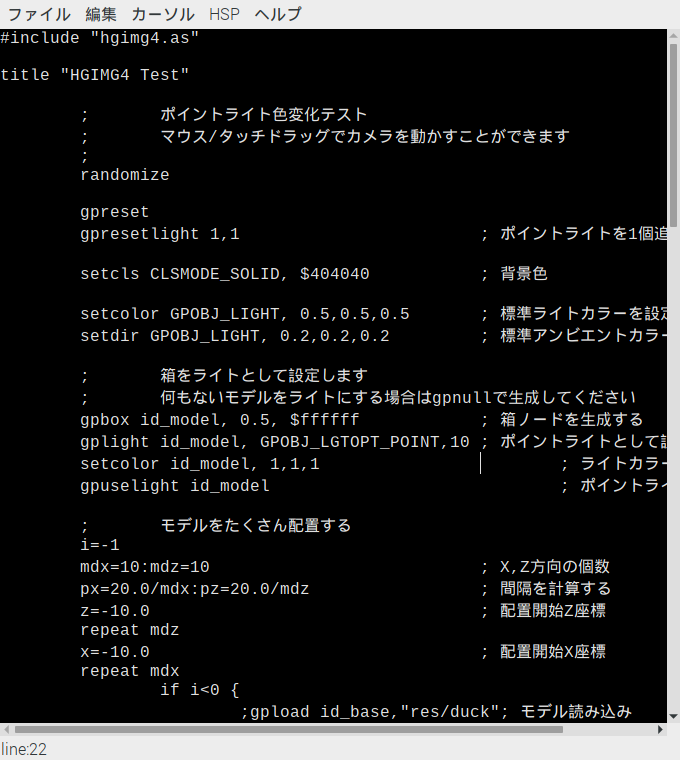
\includegraphics[keepaspectratio,width=10.971cm,height=8.229cm]{text04-img/s_lighttest3s.png}
\flushleft

Figure \stepcounter{Figure}{\theFigure}: light\_test3s.hspのプログラム}
\end{minipage}

\bigskip
\bigskip
\bigskip

[F5]キーで実行すると絵が動きます。

3D表現の画面を出す場合でも、プログラミングの方法は変わりません。ただし、今まで「横」「縦」という2つの軸があったものが、「横」「縦」「奥行き」という3つの軸に増えて、絵を出す方法も複雑になります。

\bigskip
\bigskip

\begin{minipage}{9.781cm}
\centering
{\upshape
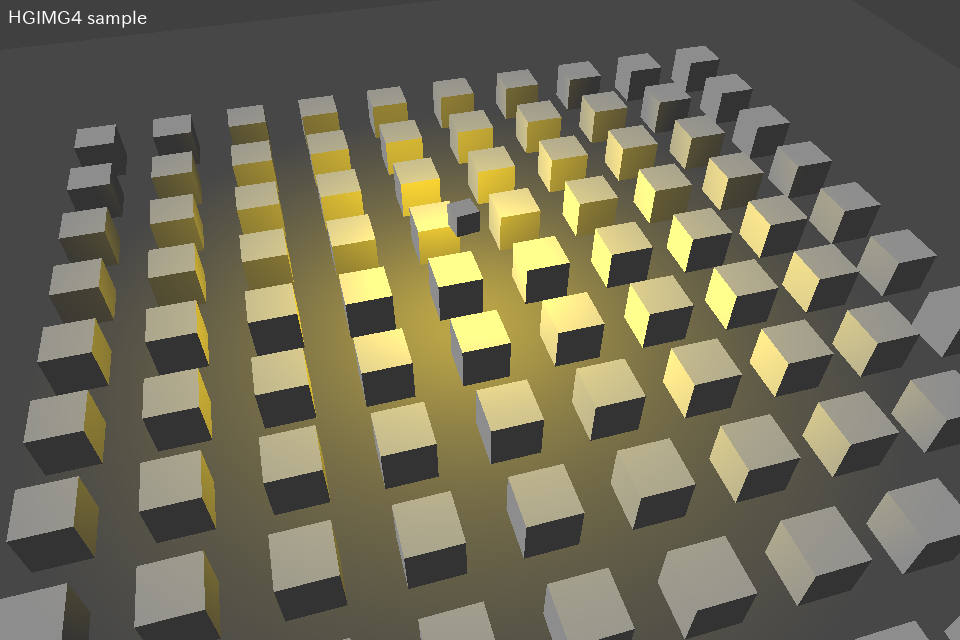
\includegraphics[keepaspectratio,width=10.971cm,height=8.229cm]{text04-img/s_lighttest3.png}
\flushleft

Figure \stepcounter{Figure}{\theFigure}: light\_test3.hspの実行画面}
\end{minipage}

\bigskip
\bigskip
\bigskip

変数や条件判断といった基本的な要素は変わらないので、皆さんはまず「2D」のやり方をよく覚えて、さらにそこからステップアップすることをおすすめします。

もう1つ、立体的なキャラクターを出すプログラムを見てみましょう。


ファイル→「開く」メニューから「/home/ユーザー名/sample/pronama3d」内の「pronama2.hsp」を読み込んでください。

[F5]キーで実行するとプロ生ちゃんというキャラクターがダンスする画面になります。

\bigskip
\bigskip

\begin{minipage}{9.781cm}
\centering
{\upshape
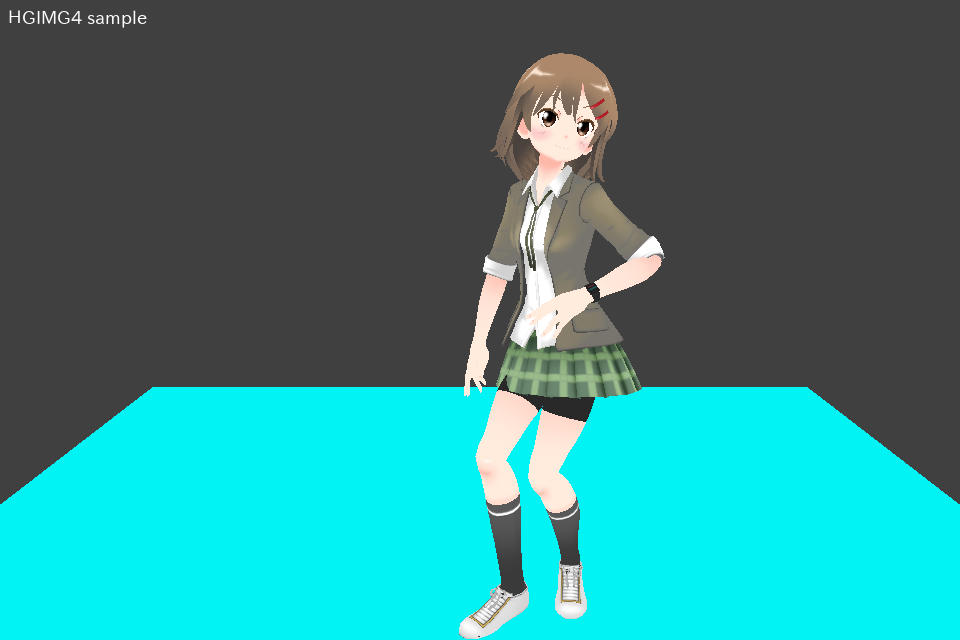
\includegraphics[keepaspectratio,width=10.971cm,height=8.229cm]{text04-img/s_pronama2.png}
\flushleft

Figure \stepcounter{Figure}{\theFigure}: pronama2.hspの実行画面}
\end{minipage}

\bigskip
\bigskip
\bigskip

立体的な絵は、GIMPのような絵を描くツールではなく、3Dグラフィックツールと呼ばれる、形そのものを細かく決めるツールによって作られています。これは、2Dの絵を描くよりもずっと難しい作業です。しかし、仕組みがわかって学習すれば作れるものでもあるのです。

\bigskip

皆さんが使っているラズベリーパイは、スマホやPCと同じような3D表示にも対応した高性能なコンピュータです。

応用によって本格的なゲームも遊べますし、それを作りだすこともできることを覚えておいてください。

\bigskip
\bigskip

\begin{minipage}{9.781cm}
\centering
{\upshape
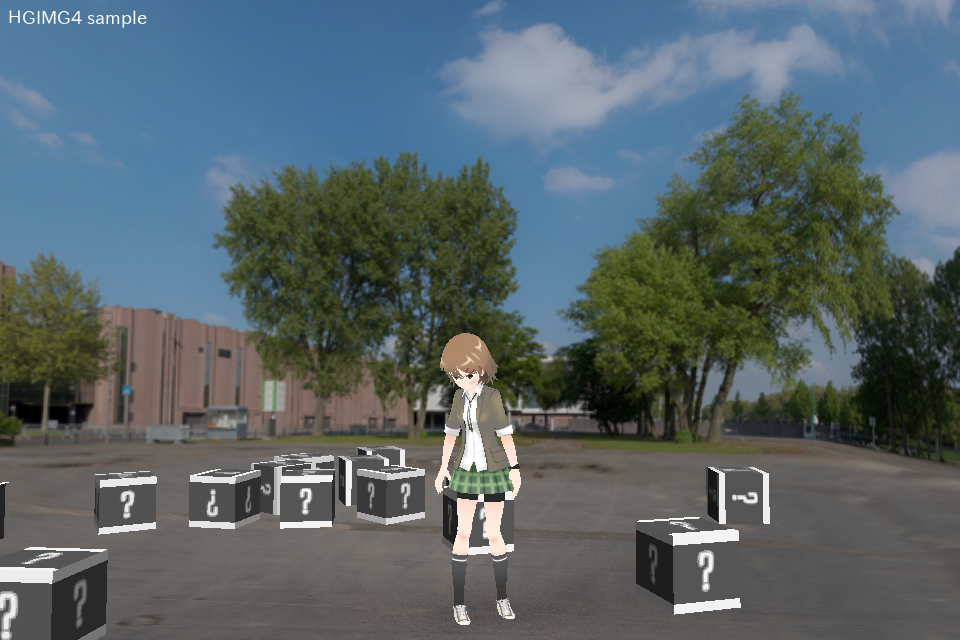
\includegraphics[keepaspectratio,width=10.834cm,height=7.514cm]{text04-img/s_pronamabox.png}
\flushleft

Figure \stepcounter{Figure}{\theFigure}: 背景とキャラクターを同時に出した画面}
\end{minipage}

\bigskip
\bigskip
\bigskip

\clearpage
\subsection{たくさんの絵を同時に動かす}
\bigskip
\bigskip

以前に、変数に横・縦の位置を代入してpos命令で指定することで絵を動かすプログラムを実行しました。変数を使うことで、絵を動かしたり、条件判断ができることはわかりました。

でも、ゲームの中では、同時にたくさんの絵を動かしています。

たくさんの敵が出てきたり、ミサイルが同時に何発も発射されたりします。これを変数で1つ1つ記憶させるためには、それだけ多くの変数を作る必要があります。

変数x、変数yが横・縦の位置を入れておくものだとして、もう1つまた変数x2、変数y2…など違う名前をつけなければなりません。

もし100個の絵を出すとすると、x100とかすごい数を書く必要があるのでしょうか…?


\bigskip

実は、これを簡単にできるような仕組みが用意されています。それが「配列変数」と呼ばれるものです。

変数はx,yなどの名前を付けた箱に数字を入れてありました。この箱に番号を付けて管理できるようにしたものが配列変数です。

変数xの1番目、2番目、3番目…といった感じで、変数の名前は同じで、番号ごとに違う内容を記憶させておくことができます。配列変数を使う時には、「(カッコ)」の中に番号を書きます。


\bigskip

{\bfseries
\ \ 変数 ( 番号 )}


\bigskip

たとえば、変数xの1番目は、x(1)のように書きます。x(1)とx(2)は別々な数字を覚えさせることができます。後は、いままでの変数と使い方は変わりません。ですから、


\bigskip

{\bfseries
\ \ x(1) = 100

\ \ x(2) = 200

\ \ x(3) = 400}


\bigskip

のようにいくつも変数xの配列変数に代入することができます。

カッコの中の番号は、0から始まって好きな数まで入れていくことができます。この番号を配列要素と呼んでいます。番号は実は、数字だけでなく変数を使うことができます。つまり、


\bigskip

{\bfseries
\ \ a=3

\ \ x(a) = 500}


\bigskip

と書いた場合は、x(3)に500という数字が代入されます。

同じ変数に複数の値が入るということで、ちょっと難しいですが、これを使うことで同時に絵を動かすことができるようになります。


\bigskip

ファイル→「開く」メニューから「array.hsp」を読み込んでください。

[F5]キーで実行すると、同時に小さな絵が動きます。

\bigskip
\bigskip

\begin{minipage}{9.781cm}
\centering
{\upshape
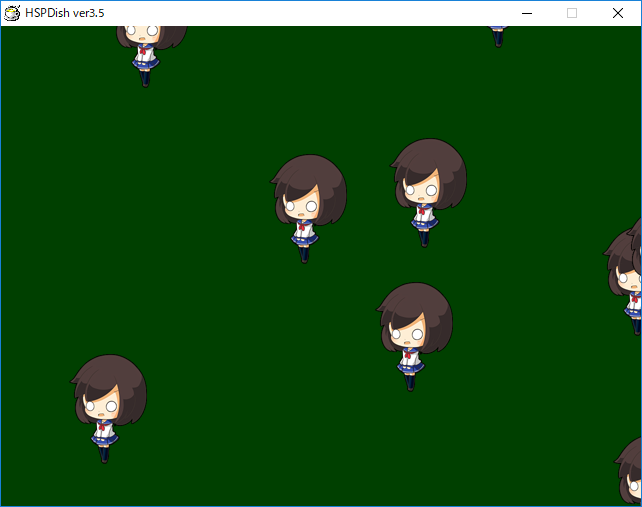
\includegraphics[keepaspectratio,width=8.811cm,height=6.946cm]{text04-img/text04-img036.png}
\flushleft

Figure \stepcounter{Figure}{\theFigure}: array.hspの実行画面}
\end{minipage}

\bigskip
\bigskip
\bigskip

ここでは、10個の絵を同時に動かしています。

最初の絵はx(0)とy(0)、次の絵はx(1)とy(1)…という感じに、変数x,yに番号をつけて複数の物体を管理しています。次のようにrepeat命令とloop命令による繰り返しを使うことで、さらに便利に配列変数を使うことができます。


\bigskip

{\bfseries
\ \ repeat 10\ \ \ \ ; 10回繰り返し

\ \ \ \ pos x(cnt),y(cnt)\ \ ; 表示位置を設定する

\ \ \ \ celput 1\ \ \ \ ; 画像を描画する

\ \ loop\ \ \ \ \ \ ; 繰り返し終わり}


\bigskip

repeat〜loop命令で繰り返している間は、システム変数cntが0,1,2…と順番に変化します。これを使って配列の要素を切り替えながら、それぞれの座標に描画することになります。


\bigskip

自分なりにプログラムを改造しながら、どのように変化するか確認してみましょう。

今は10個の絵を動かしていますが、もっと多くするにはどうすればいいか考えてみましょう。


\clearpage
\subsection{キーボードで絵を動かしてみよう}
\bigskip
\bigskip

スクリプトエディタの、ファイル→「開く」メニューから「move.hsp」を読み込んで実行してみてください。

\bigskip
\bigskip

\begin{minipage}{9.781cm}
\centering
{\upshape
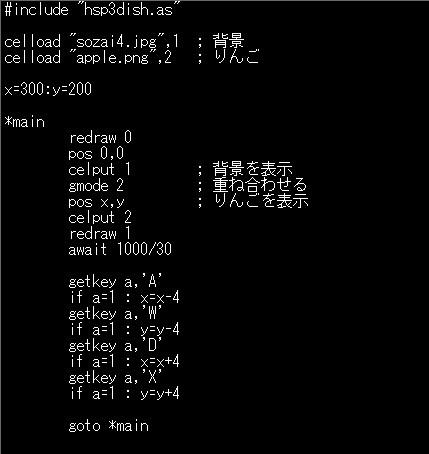
\includegraphics[keepaspectratio,width=10.61cm,height=11.229cm]{text04-img/text04-img037.png}
\flushleft

Figure \stepcounter{Figure}{\theFigure}: move.hspの実行画面}
\end{minipage}

\bigskip
\bigskip
\bigskip

これは背景とりんごを表示するプログラムですが、リンゴを「A」「W」「D」「X」のキーを押して動かすことができます。何だかゲームみたいですね。


\bigskip

りんごをどのように動かしているのでしょうか。

いままでは、「x=x+2」のような行を入れて、1コマずつ動かしていました。

今度は、キーボードのボタンを押している時だけ、動くようにすればいいのです。

そのために、以前にも使った条件判断の仕組みを利用します。


\bigskip

キーボードが押されているかどうかを条件判断するために、新しい命令、getkeyの使い方を覚えておきましょう。


\bigskip

{\bfseries
\ \ getkey 変数 , ‘キーの文字’}


\bigskip

と書くことで、指定した変数にキーが押されたかどうかが数値として代入されます。

たとえば、


\bigskip

{\bfseries
\ \ getkey a, ‘X’}


\bigskip

を実行すると、「X」キーの状態で変数aの値が0か1になります。

{\bfseries
「X」のキーが押されていない時は、変数aは0になります。

「X」のキーが押されている時は、変数aは1になります。}

\bigskip

キーの文字は、必ず大文字で’A’のように書く必要があるので注意してください。

文字の代わりにキーコードと呼ばれる数字を指定することで、特殊なキーの状態を知ることもできます。


\bigskip

{\bfseries
\ \ キーコード : 実際のキー

\ {}-{}-{}-{}-{}-{}-{}-{}-{}-{}-{}-{}-{}-{}-{}-{}-{}-{}-{}-{}-{}-{}-{}-{}-{}-{}-{}-{}-{}-{}-{}-{}-{}-{}-{}-{}-{}-{}-{}-{}-{}-{}-

\ \ \ \ \ \ \ \ 1 \ \ \ : マウスの左ボタン

\ \ \ \ \ \ \ \ 2 \ \ \ : マウスの右ボタン

\ \ \ \ \ \ \ \ 8 \ \ \ : [BACKSPACE]

\ \ \ \ \ \ \ \ 9 \ \ \ : [TAB]

\ \ \ \ \ \ \ 13 \ \ \ : [ENTER]

\ \ \ \ \ \ \ 16 \ \ \ : [SHIFT]

\ \ \ \ \ \ \ 17 \ \ \ : [CTRL]

\ \ \ \ \ \ \ 18 \ \ \ : [ALT]

\ \ \ \ \ \ \ 32 \ \ \ : スペースキー

\ \ \ \ \ \ \ 37 \ \ \ : カーソルキー[←]

\ \ \ \ \ \ \ 38 \ \ \ : カーソルキー[↑]

\ \ \ \ \ \ \ 39 \ \ \ : カーソルキー[→]

\ \ \ \ \ \ \ 40 \ \ \ : カーソルキー[↓]

\ \ \ 48〜57 \ \ \ : [0]〜[9](メインキーボード)

\ \ \ 65〜90 \ \ \ : [A]〜[Z]

\ \ 96〜105 \ \ \ : [0]〜[9](テンキー)

\ 112〜121 \ \ \ : ファンクションキー [F1]〜[F10]}

\bigskip

こうして代入された0か1の値を条件判断によって、やりたい内容を書くことで色々なことに応用ができます。

\clearpage

\bigskip

条件判断の方法をもう一度思い出してください。

if命令の使い方、ルールを覚えていますか?


\bigskip

{\bfseries
\ \ (HSPのルール)

\bigskip

\ \ if命令により条件を判断することができる

\ \ ifの後にスペースに続けて条件式を指定します

\ \ その後で「:」に続けて条件が正しい時に実行される命令を書きます}

\bigskip

\ \ (条件式はいくつか書き方があります)


\bigskip

\ \ \ \ 条件式 \ \ \ \ \ \ \ \ \ 意味

\ \ \ \ {}-{}-{}-{}-{}-{}-{}-{}-{}-{}-{}-{}-{}-{}-{}-{}-{}-{}-{}-{}-{}-{}-{}-{}-{}-{}-{}-{}-{}-{}-{}-{}-{}-{}-{}-{}-{}-{}-{}-{}-{}-{}-{}-{}-{}-{}-{}-{}-{}-{}-{}-{}-

\ \ \ \ 変数名 =
数値\ \ 変数の内容と数値が同じである

\ \ \ \ 変数名 !
数値\ \ 変数の内容と数値が同じではない

\ \ \ \ 変数名 {\textless}
数値\ \ 変数の内容より数値の方が大きい

\ \ \ \ 変数名 {\textgreater}
数値\ \ 変数の内容より数値の方が小さい


\bigskip

下のプログラムがどのような意味か考えてみましょう。


\bigskip

{\bfseries
\ \ getkey a,’A’

\ \ if a=1 : x=x-4}


\bigskip

最初は、条件判断の仕組みがわかりにくいかもしれませんが、プログラムの1行目から、コンピューターが実行することを想像しながら、1つ1つ確認することが大切です。

やがて、プログラムを見て、どのように動くのか想像ができるようになります。

最初はちょっと難しく感じるかもしれませんが、慣れれば誰でも理解できるようになります。

あせらず、わからない所はまわりの先生や友達に聞きながら、進んでいきましょう。

\bigskip

\subsection{例題に挑戦しよう}

\bigskip
\bigskip

ゲームが遊べた人は、以下の例題にも挑戦してみよう。

\bigskip

・センサーボードのボタンを使ってみよう

・照度センサーの値をもとに絵を動かそう

・照度センサーを使ったゲームを遊んでみよう

・センサーボードを使った応用例を考えてみよう


\bigskip

例題の考え方がわからない時は、近くのTAか先生に聞いてください。

わからない所は、そのままにせず、必ず答えを見つけてから先に進みましょう。

\clearpage
\subsection{例題4-12 センサーボードの入力を使ってみよう}
\bigskip
\bigskip

{\bfseries
考え方}

\bigskip

キーボードの代わりにセンサーボードのボタンを使って絵を動かしてみましょう。

move.hspのプログラムを改造して、センサーボードのボタンで絵を動かせるようにしましょう。

\bigskip
\bigskip

\begin{minipage}{9.781cm}
\centering
{\upshape
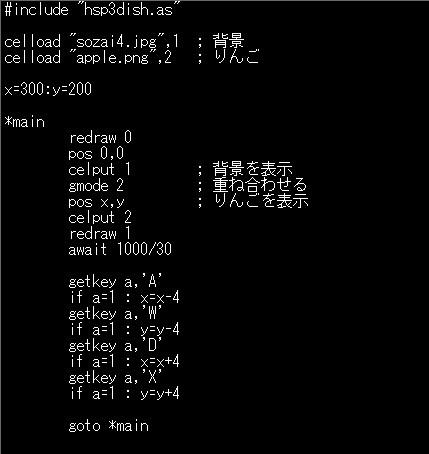
\includegraphics[keepaspectratio,width=10.61cm,height=11.229cm]{text04-img/text04-img037.png}}
\end{minipage}

\bigskip
\bigskip
\bigskip

{\bfseries
例題4-12 答え}


\bigskip

以前に取り上げた、GPIOの番号とその役割を思い出してみてください。

\bigskip
\bigskip

\begin{minipage}{9.781cm}
\centering
{\upshape
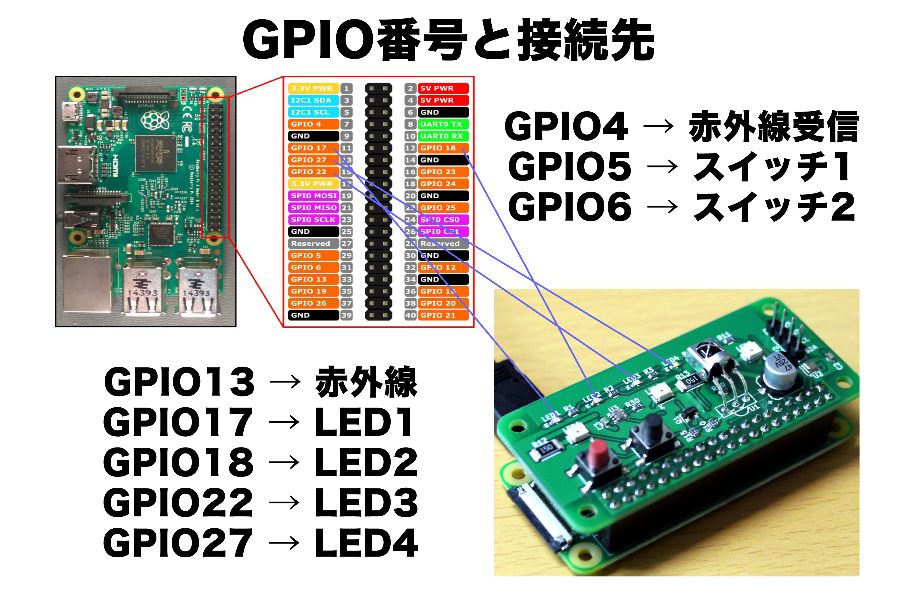
\includegraphics[keepaspectratio,width=10.372cm,height=6.89cm]{text04-img/text04-img004.png}}
\end{minipage}

\bigskip
\bigskip
\bigskip

スイッチの状態などを知る場合は、gpioinという関数を使います。


\bigskip

{\bfseries
\ \ 変数 = gpioin(GPIO番号)}


\bigskip

と書くことで、指定されたGPIO番号のスイッチがONかOFFかを調べることができます。

変数には0か1の数字が代入されるので、条件判断を行うif命令で違う動作をさせることができます。


\bigskip

{\bfseries
\ \ a = gpioin(5)

\ \ if a=0 : x=x-4}


\bigskip

のように書くことで、変数aが0の時だけ「x=x-4」を実行させることができます。


\bigskip

以下のようにプログラムを改造することで、センサーボードのボタンを条件判断で使うことができます。

\bigskip
\bigskip

\begin{minipage}{9.781cm}
\centering
{\upshape
\includegraphics[keepaspectratio]{text04-img/text04-img038.png}}
\end{minipage}

\bigskip
\bigskip
\bigskip

改造ができたらTAや周りの友達にも見せてあげましょう。

\bigskip

以前に乱数の使い方を学習したことを思い出してみましょう。

「x=rnd(640)」は、0〜639(640通り)までのバラバラな数字を変数xに代入します。

このような書き方を「乱数」と呼んでいます。


\bigskip
\bigskip

\begin{minipage}{9.781cm}
\centering
{\upshape
\includegraphics[keepaspectratio,width=11.906cm,height=5.662cm]{text04-img/text04-img039.png}}
\end{minipage}

\bigskip
\bigskip
\bigskip

{\bfseries
\ \ (HSPのルール)

\bigskip

\ \ 「変数=rnd(乱数の最大値)」でバラバラな数字を得ることができる

\ \ 関数は、「変数=関数(パラメーター)」という書き方で使うことができる}

\bigskip

乱数が代入された変数を条件判断することで、でたらめな動きをする絵を作ることもできます。

余裕がある人は、乱数を使った動きにも挑戦してみましょう。


\clearpage
\subsection{例題4-13 照度センサーの値をもとに絵を動かそう}
\bigskip
\bigskip

{\bfseries
考え方}

\bigskip

センサーボードのボタンだけでなく、照度センサーを使うこともできます。

照度センサーがどのような機能を持っているか、確認しておきましょう。


\bigskip

ファイル→「開く」メニューから「luxmove.hsp」を読み込んでください。

[F5]キーで実行すると、照度センサーの値が表示されると同時に小さな絵が動きます。

\bigskip
\bigskip

\begin{minipage}{9.781cm}
\centering
{\upshape
\includegraphics[keepaspectratio,width=11.615cm,height=10.94cm]{text04-img/text04-img040.png}}
\end{minipage}

\bigskip
\bigskip
\bigskip

左上に表示されている数値が照度センサーの値です。

明るい時ほど大きい数字になるのがわかりますか?

自分の手でセンサーを覆ったり、光を当ててみたりしながら値が変わることを確認してみましょう。


\bigskip

確認ができたら、move.hspのプログラムを改造して、りんごの絵を照度センサーの値によって動かせるようにしてみましょう。


\bigskip

{\bfseries
例題4-13 答え}


\bigskip

「geti2c\_lux\_init」命令を最初に入れて1回だけ初期化を行います。

その後、一定時間ごとに「geti2c\_lux」命令を実行することで、rpz\_luxという変数にセンサーの値が代入されます。

後は、rpz\_luxという変数の値をもとにプログラムで処理を行います。


\bigskip

改造ができたらTAや周りの友達にも見せてあげましょう。


\clearpage
\subsection{例題4-14 照度センサーを使ったゲームを遊んでみよう}
\bigskip
\bigskip

{\bfseries
考え方}

\bigskip

アイデア次第で、キーボードだけでなく、センサー類を使ってゲームのようにすることができます。

光センサーを使ったゲームを動かしてみましょう。


\bigskip

スクリプトエディタの、ファイル→「開く」メニューから「catch.hsp」を読み込んで実行してみてください。


\bigskip


\bigskip

{\bfseries
例題4-14 答え}


\bigskip

センサーボードの光センサーから得た値を使って絵を動かしています。光センサーを手で覆ったり、離したりしてどうなるか確認してみましょう。

光センサーが暗くなった時には、キャラクターが左に移動します。光センサーが明るくなった時には、キャラクターが右に移動します。

\bigskip
\bigskip

\begin{minipage}{9.781cm}
\centering
{\upshape
\includegraphics[keepaspectratio,width=11.269cm,height=8.89cm]{text04-img/text04-img041.png}
\flushleft

Figure \stepcounter{Figure}{\theFigure}: catch.hspの実行画面}
\end{minipage}

\bigskip
\bigskip
\bigskip

うまくキャラクターを移動させて、上から落ちてくるリンゴをキャッチしてみましょう。


\bigskip

これは、いままでの応用ですが、センサーと動きのある画面を組み合わせるだけでも、面白いものが作れるはずです。gpio命令で、LEDを光らせたり、スイッチを読み取ったりということと、変数・条件判断を組み合わせれば、さらに応用範囲が広がります。

\clearpage
\subsection{例題4-15 センサーボードを使った応用例を考えてみよう}
\bigskip
\bigskip

{\bfseries
考え方}

\bigskip

今まで覚えてきたことを組み合わせて、何ができるか考えてみましょう。家に帰ってから、考えてみて答えを書いてきてください。センサーボードで何ができるか、プログラムでどんなことができるか、もう一度思い出してみて、考えてみましょう。

考えがまとまらない人は、いままでに動かしたプログラムを改造してみたいこと、センサーボードでやってみたいことを書いてみましょう。実際にプログラムを作る必要はありません。いっぱい考えついた人は、例題4-16と例題4-17の答えの欄に書いてみましょう。


\bigskip

大切なことは、自分で何でも試してみることです。わからないことがあっても、実際に実行すれば結果がわかります。立ち止まらずに、どうなるか想像しながらプログラムを書いて実行することが、早く上達するコツになります。それでもわからない時は、先生に聞いてみましょう。


\bigskip

{\bfseries
例題4-15 答え}


\bigskip

自分で考えた応用例を下に書いておきましょう。

応用例ができたら、今まで覚えてきた命令でできることか考えてみましょう。

実際に作れる人は、自分でプログラムを作ってみてください。


\clearpage
\subsection{例題4-16 センサーボードの応用例をもっと考えてみよう(1)}
\bigskip
\bigskip

{\bfseries
例題4-16 答え}


\bigskip


\bigskip


\bigskip


\bigskip


\bigskip


\bigskip


\bigskip


\clearpage
\subsection{例題4-17 センサーボードの応用例をもっと考えてみよう(2)}
\bigskip
\bigskip

{\bfseries
例題4-17 答え}


\bigskip


\bigskip


\bigskip


\bigskip


\bigskip


\bigskip


\bigskip



  % Last Part:

\clearpage\section{質問フォーム}
わからないこと、質問したいことがあれば質問フォームから質問しよう!

質問フォームでは、授業でわからなかったことや確認(かくにん)したいことなどをホームページを通して質問できます。たくさん質問してわからないことを解決しよう。

\bigskip

\bigskip

1.
ブラウザで\textbf{授業で使うホームページリスト}を開こう。

\bigskip

\textbf{授業で使うホームページリスト}は/home/ユーザー名/01フォルダの中のlinks.htmlです

リストの4番目の子ども\textbf{IT未来塾質問フォーム}をクリックして開いてください(Figure~\ref{seq:refFigure46})。


\bigskip

{\bfseries
スマートフォン等からの場合は\url{https://bit.ly/2NHiVgi}を開いてください。}



\begin{minipage}{9.781cm}
\centering
{\upshape
\includegraphics[width=11.231cm,height=7.613cm]{textbook-img245.png}
\flushleft

\bigskip
Figure {\refstepcounter{Figure}\theFigure\label{seq:refFigure46}}:
ホームページリストより質問フォームを開く}
\end{minipage}

\bigskip

\bigskip

2.
質問フォーム(Figure~\ref{seq:refFigure47})が表示されます

\centering
\begin{minipage}{11.915cm}
{\upshape
\includegraphics[width=13.263cm,height=14.233cm]{textbook-img246.png}
\flushleft

\bigskip
Figure {\refstepcounter{Figure}\theFigure\label{seq:refFigure47}}: 質問フォーム}
\end{minipage}
\flushleft

\bigskip

メールアドレス、お名前、グループの先生の名前、ぎもんに思っていることを入力します。必要に応じて、ぎもんに思っている場所の画像を追加してください。

{\bfseries
送信\textmd{を押すと質問ができます。Figure~\ref{seq:refFigure48}の画面が出たら質問は完了です。}}



\centering
\begin{minipage}{8.871cm}
{\upshape
\includegraphics[width=8.871cm,height=4.374cm]{textbook-img247.png}
\flushleft

\bigskip
Figure {\refstepcounter{Figure}\theFigure\label{seq:refFigure48}}: 質問送信画面}
\end{minipage}
\flushleft
メールアドレスのらんに入力したアドレスへグループの先生から回答メールがきます。
メールが来るまで、しばらくお待ちください。数日かかる場合があります。

\end{document}
